%\clearpage
\renewcommand{\thefigure}{S\arabic{figure}}
\renewcommand{\thetable}{S\arabic{table}}
\renewcommand{\theequation}{S\arabic{equation}}
\renewcommand{\thesection}{}
\renewcommand{\thesubsection}{S\arabic{subsection}}
\setcounter{figure}{0}
\setcounter{table}{0}
\setcounter{section}{0}
\setcounter{equation}{0}

%\resetlinenumber
%\input sipre.tex
%\section*{Supporting Information}
\label{sec:sm}
\renewcommand{\thepage}{S\arabic{page}}
\setcounter{page}{1}
\begin{figure*}[!h]
\centering
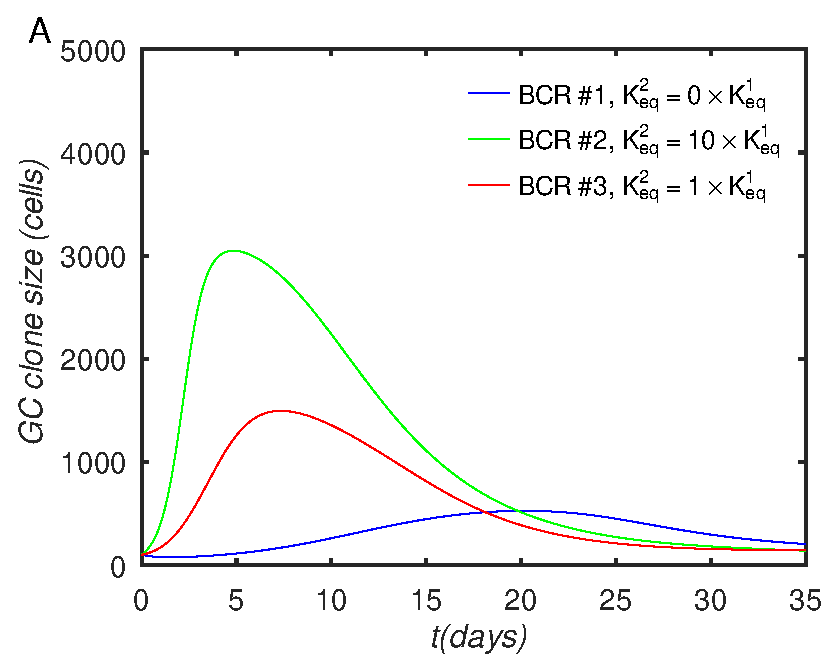
\includegraphics[width=0.45\textwidth]{../figS1abc/gcsize.eps}
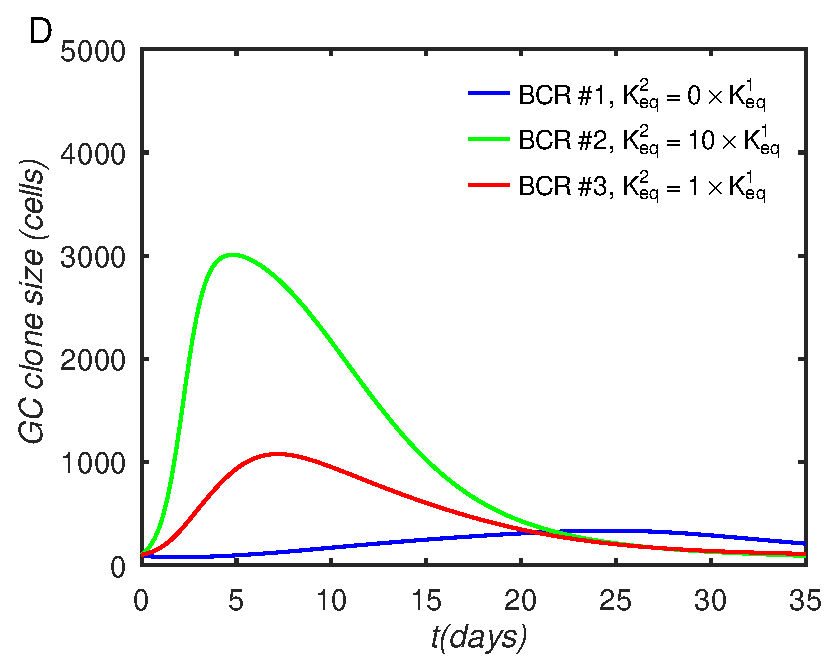
\includegraphics[width=0.45\textwidth]{../figS1def/gcsize.eps}
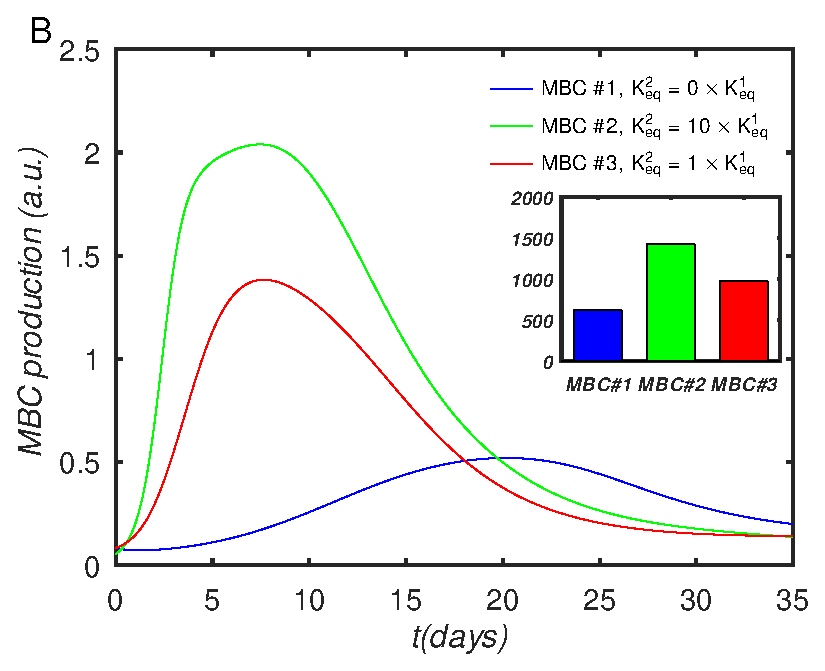
\includegraphics[width=0.45\textwidth]{../figS1abc/dmbc.eps}
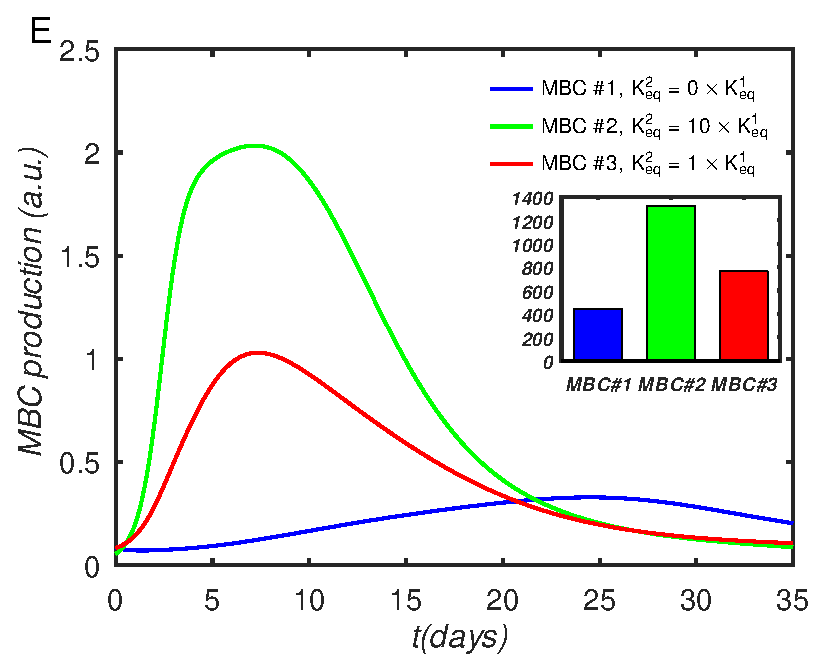
\includegraphics[width=0.45\textwidth]{../figS1def/dmbc.eps}
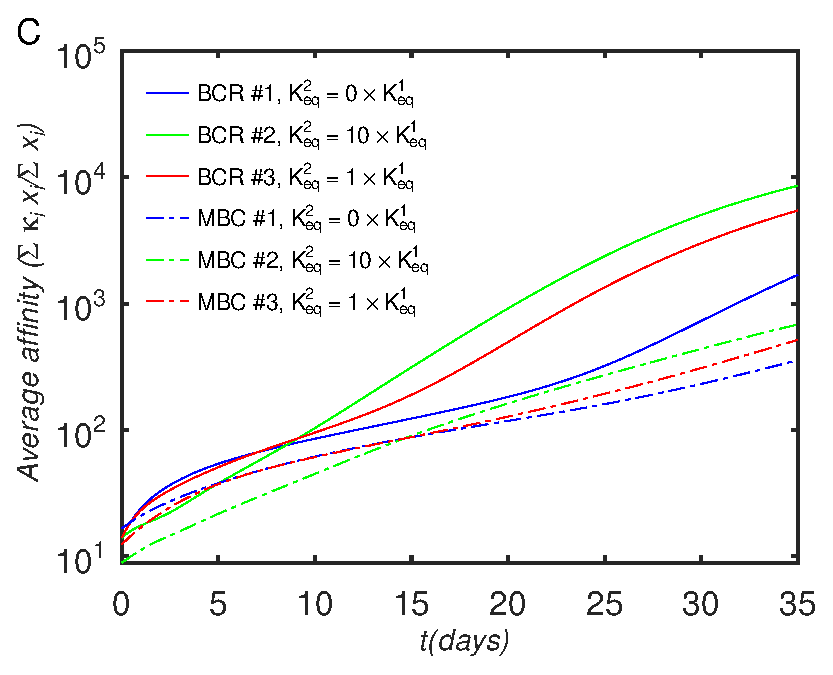
\includegraphics[width=0.45\textwidth]{../figS1abc/A.eps}
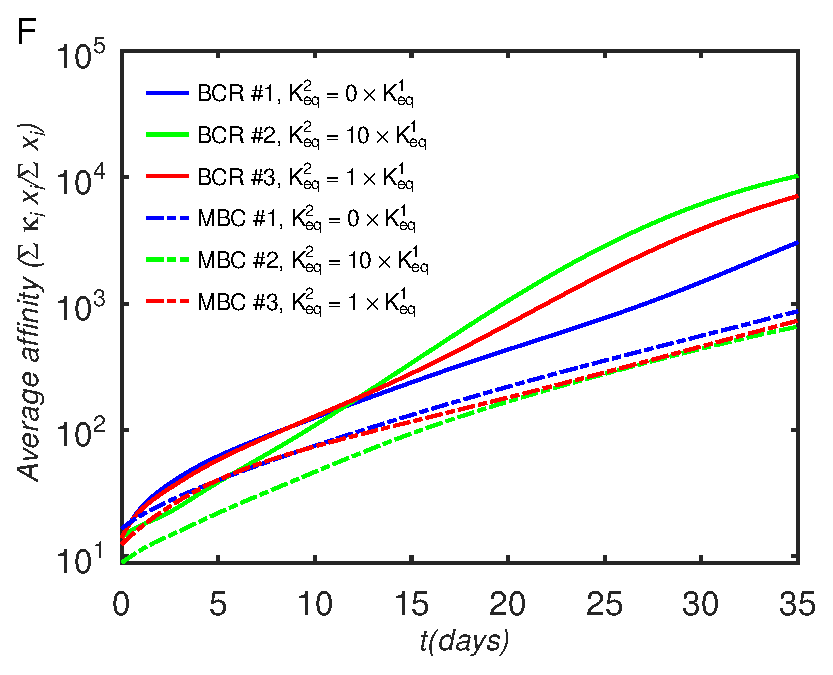
\includegraphics[width=0.45\textwidth]{../figS1def/A.eps}
\caption{Effect of antibody valency and epitope occlusion on GC properties; different B-cell clones interact in the intermediate
regime, \ie~
left column (A--C): $o=0.5$;
Right column (D--F): $o=0.9$;
A,D: Total B cells;
B,E: Memory cell production rate; insets: total MBC population at end of simulation;
C,F: Average affinity of B-cells and MBCs.
}
\label{fig:intavidity}
\end{figure*}
\begin{figure*}
\centering
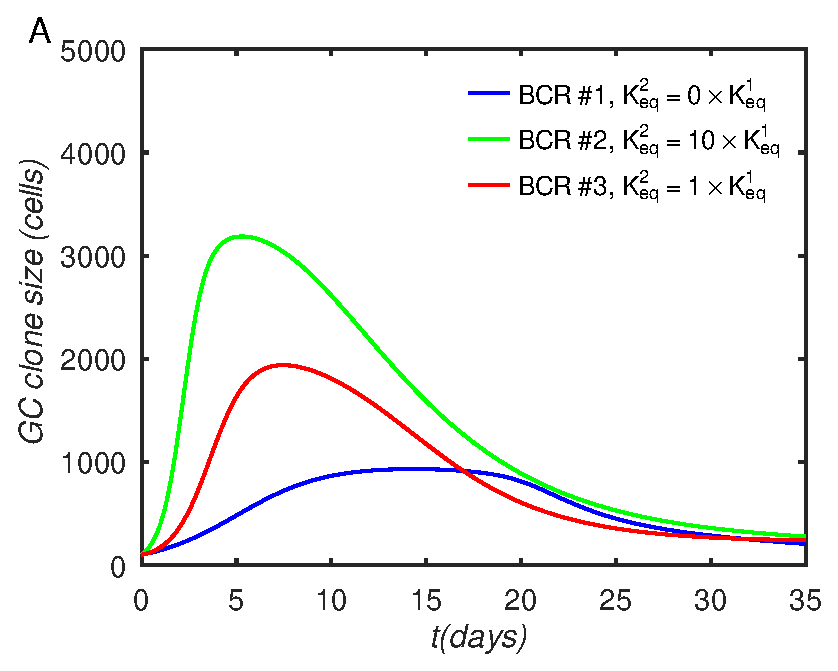
\includegraphics[width=0.32\textwidth]{../figS2/gcsize.eps}
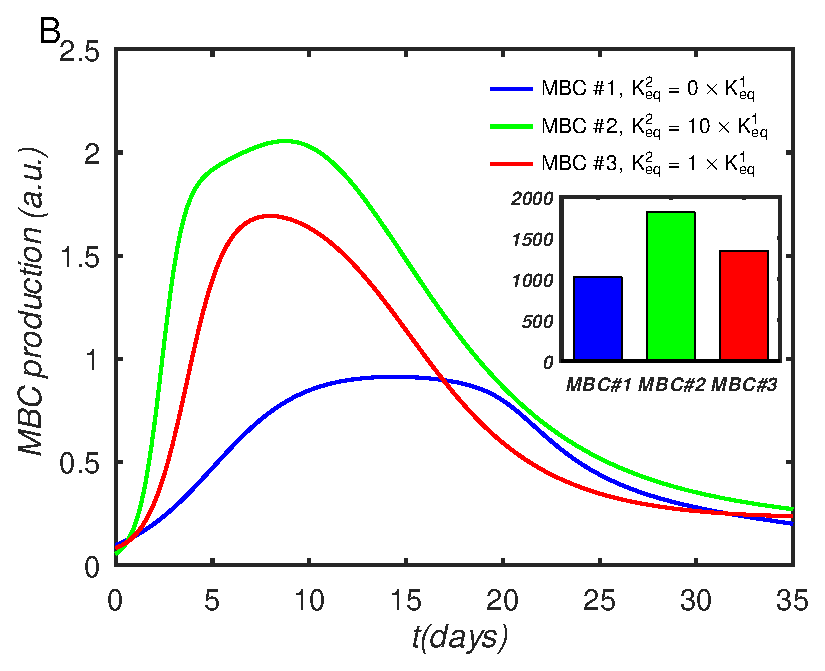
\includegraphics[width=0.32\textwidth]{../figS2/dmbc.eps}
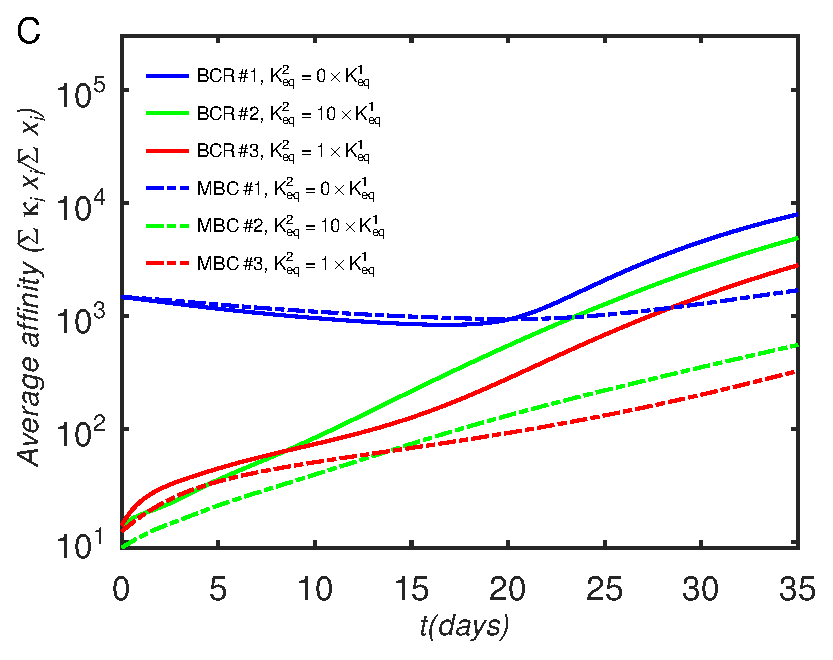
\includegraphics[width=0.32\textwidth]{../figS2/A.eps}
\caption{Effect of initial affinity advantage on the growth of monovalent B-cells in the independent
(noninteracting) B-cell case ($o=0$).
Panels A--C show the same quantities as Fig.~5A--C;
The affinity distribution corresponding to BCR\#1 was shifted toward higher values relative to BCR\#2 and BCR\#3
(Fig.~5D, main text).
}
\label{fig:kadv0}
\end{figure*}

\begin{figure*}
\centering
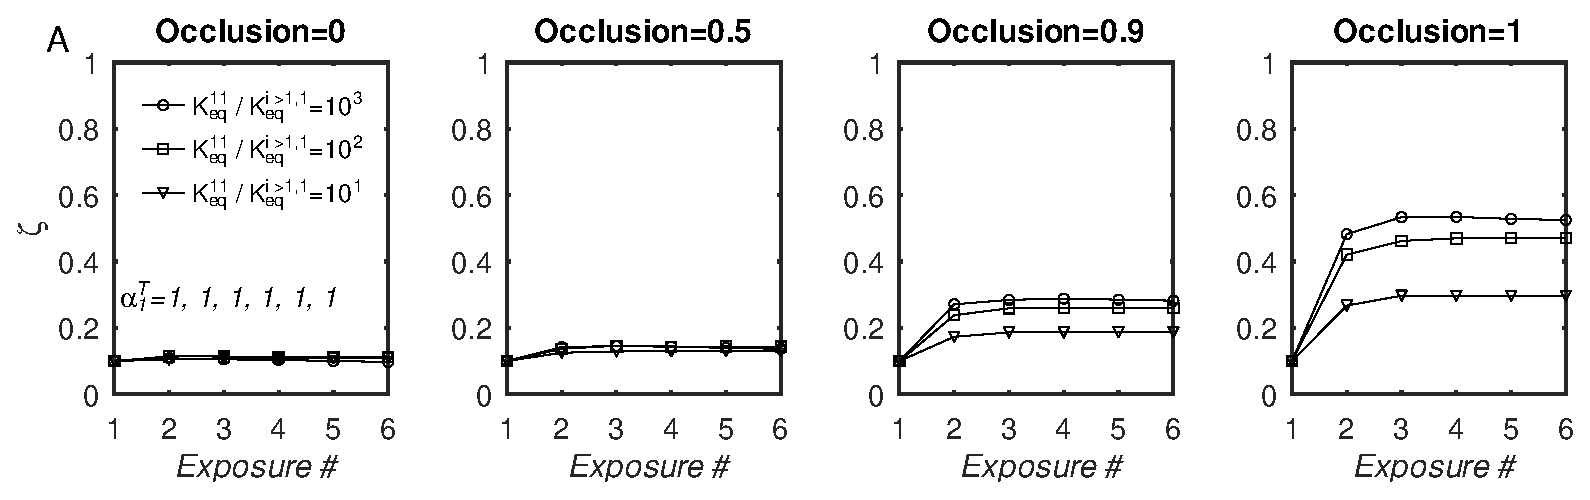
\includegraphics[width=0.99\textwidth]{../fig8-S3-S8/mbctime-k12=10si.eps}
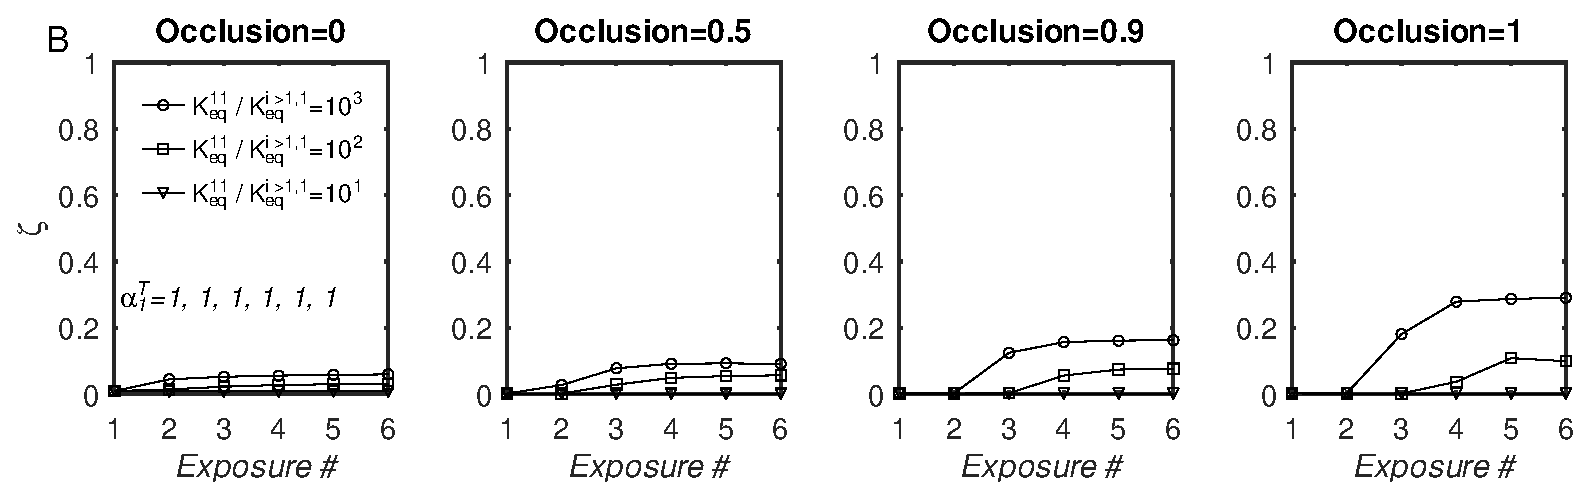
\includegraphics[width=0.99\textwidth]{../fig8-S3-S8/mbctime-k12=0si.eps}
\caption{Fraction of MBC\#1 \vs~number of sequential GC simulations for different initial affinity advantage values
 with 10 total BCR/Epitope pairs.
A: BCR\#1 is cooperatively bivalent ($K^{12}_{eq}$=10$K^{11}_{eq}$);
B: BCR\#1 is monovalent ($K^{12}_{eq}$=0).
}
\label{fig:mbctime}
\end{figure*}

\vspace{1EM}
\subsection{
GC simulations with a variable $\Delta K_{eq}$ BCR\#1 advantage}
\label{sec:fig5}
\begin{figure*}
\centering
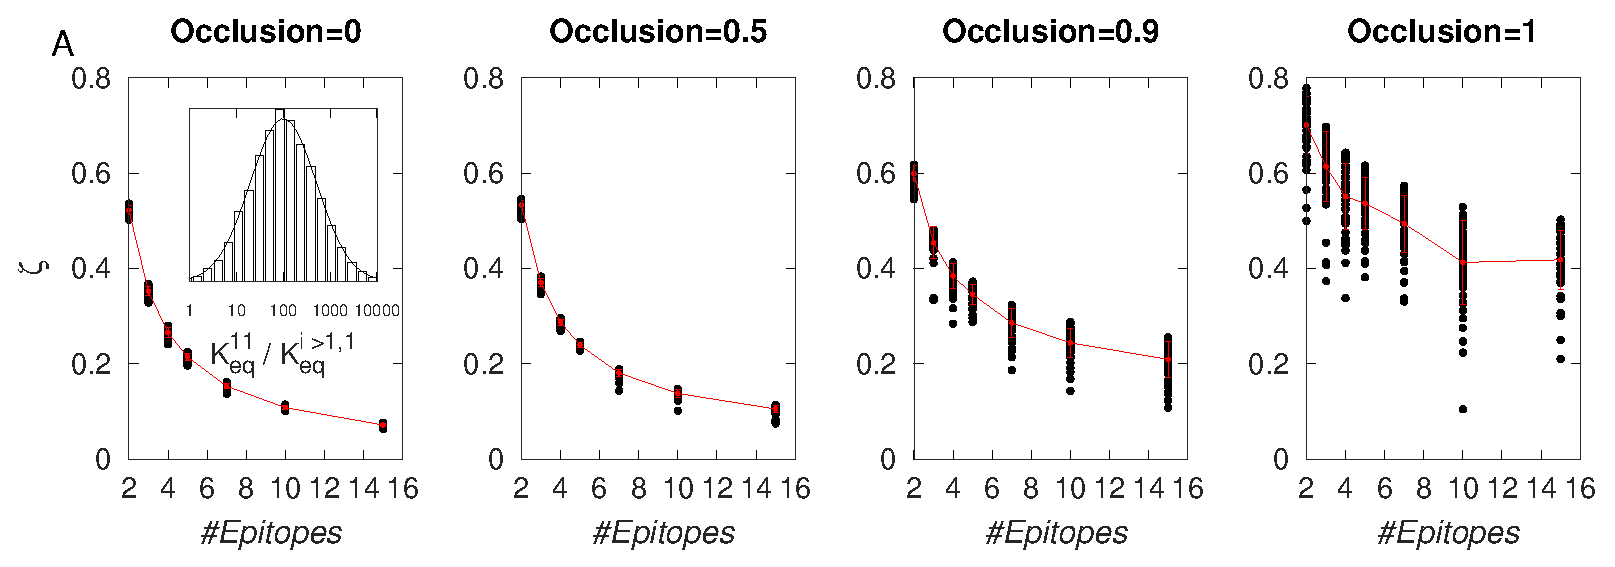
\includegraphics[width=0.99\textwidth]{../figS4/occl-k12=10rnd.eps}
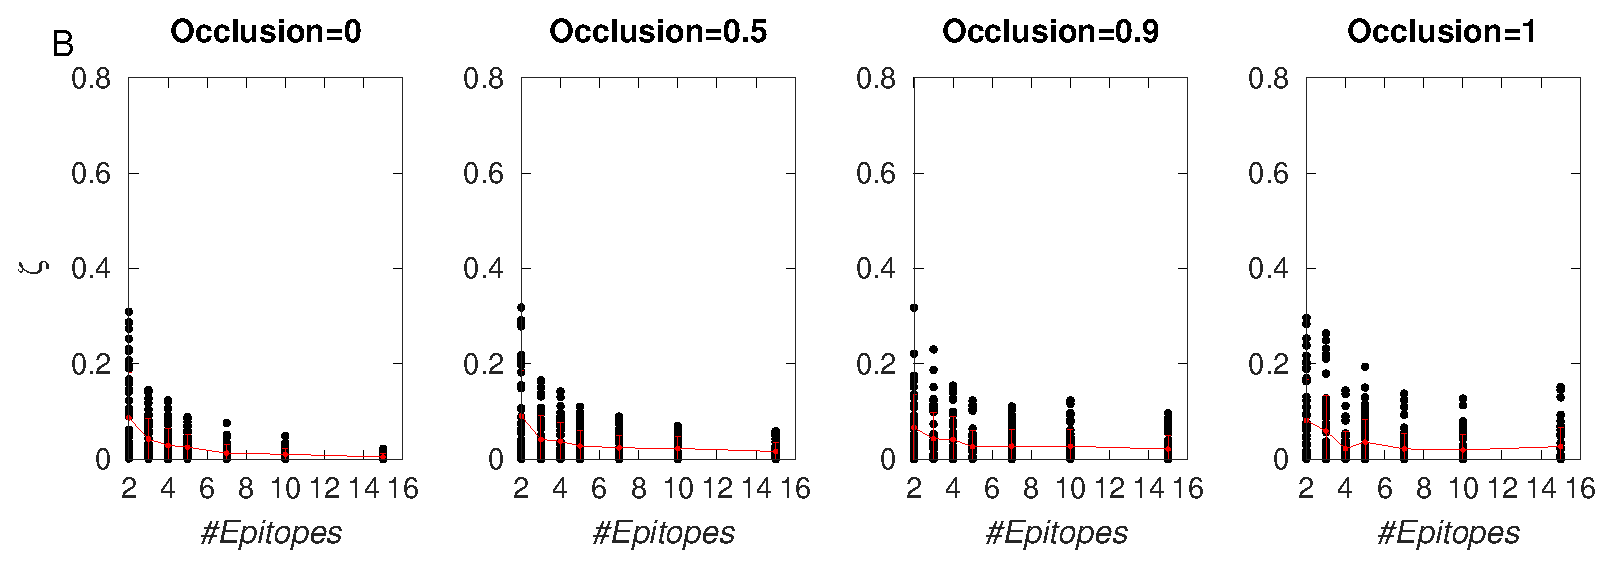
\includegraphics[width=0.99\textwidth]{../figS4/occl-k12=0rnd.eps}
\caption{Fraction of MBC\#1 at the end of six GC simulations for initial affinity advantage values drawn from the
 lognormal distribution (inset of panel A)
 \vs~total number of BCR/Epitope pairs.
A: BCR\#1 is cooperatively bivalent ($K^{12}_{eq}$=10$K^{11}_{eq}$);
B: BCR\#1 is monovalent ($K^{12}_{eq}$=0).
Red vertical bars represent standard deviation.
}
\label{fig:kadvrand}
\end{figure*}
Because the affinity advantage of a BCR targeting a conserved epitope cannot be predicted
accurately if antigenic drift is present, instead of modeling an affinity advantage of a particular BCR using a constant
$\Delta K_{eq}$, as done in the main text (see Fig.~6), a more realistic scenario is
to treat $\Delta K_{eq}$ as a random variable.
To this end, in the simulations described here we sample $\log_{10} \Delta K_{eq}$
from the Gaussian distribution centered on 2 (which corresponds to $\Delta K_{eq}$=100) with variance 0.5
; equivalently, $\Delta K_{eq}$ is sampled from the lognormal distribution.
Each set of simulations is repeated 50 times to
generate statistics. The distribution of $\Delta K_{eq}$ is shown in \fig{kadvrand}A (inset).

\Fig{kadvrand} panels A and B show the MBC\#1 fraction from the
simulations of the bivalent and monovalent cases, respectively.
The differences between the two cases are similar to those in
previous simulations with fixed $\Delta K_{eq}$. For
the bivalent case, the average MBC\#1 fraction for the competing cases $\occl\ge
0.9$, is around 30\%--40\% for 9 or more distracting epitopes, whereas
for the monovalent case, this number is on the average about 3\%. More importantly, in the
bivalent case, some MBC\#1 cells are always present, while in some individual simulations
of the monovalent case, MBC\#1 proportion is near zero (\fig{kadvrand}B).

\vspace{1EM}
\subsection{Solvent-accessible surface area of HA}
\label{sec:sasa}
\begin{figure*}
\centering
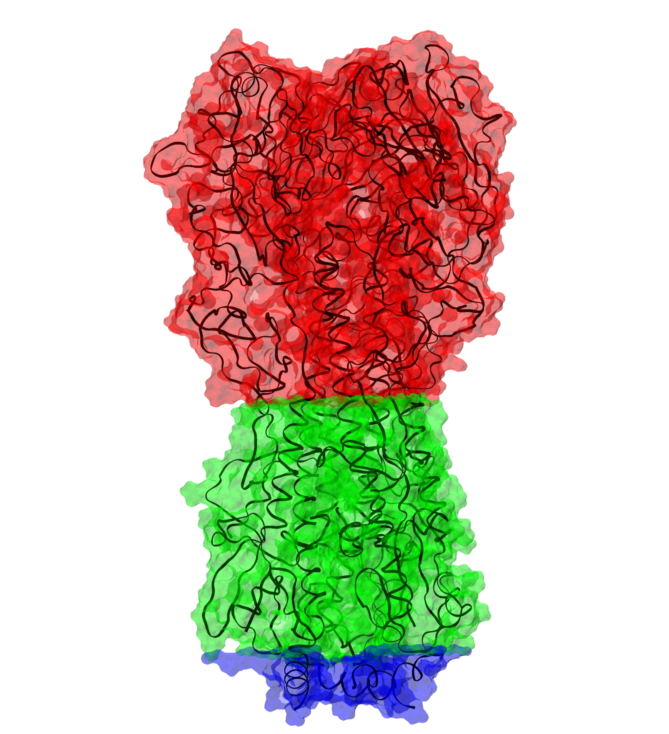
\includegraphics[width=0.3\textwidth]{fig-h1n1.png}
\caption{
Illustration of a H1N1 hemagglutinin trimeric spike partitioned into the head (red, top), stem (green, middle), and base (blue, bottom) regions.
The structure is taken from PDB entry 3LZG\cite{xu10}.
}
\label{fig:sasa}
\end{figure*}
Solvent-accessible surface areas (SASA) of the HA head, stem, and base
regions were computed using the structure of H1N1 virus
California/04/2009 from PDB entry 3LZG.\cite{xu10} The program
CHARMM\cite{Brooks09} with standard parameters\cite{Best12} and water
probe radius of 1.4\AA~was used for the SASA computation. The HA was
partitioned into three regions, head, stem, and base, as shown in
\fig{sasa} in red, green, and blue, respectively. The corresponding SASA
values were computed to be 314, 175, and 50 $nm^2$.

\begin{figure*}
\centering
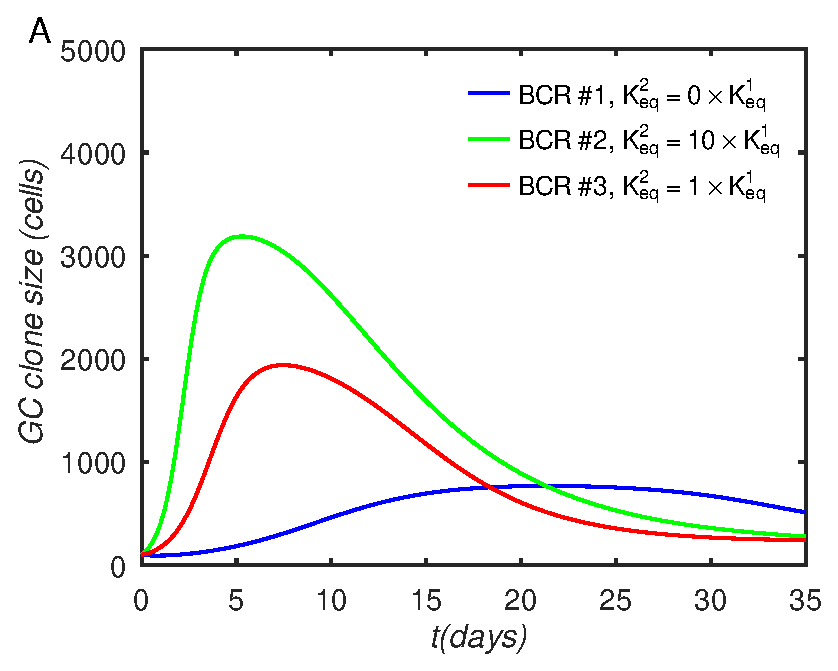
\includegraphics[width=0.49\textwidth]{../figS6/gcsize.eps}
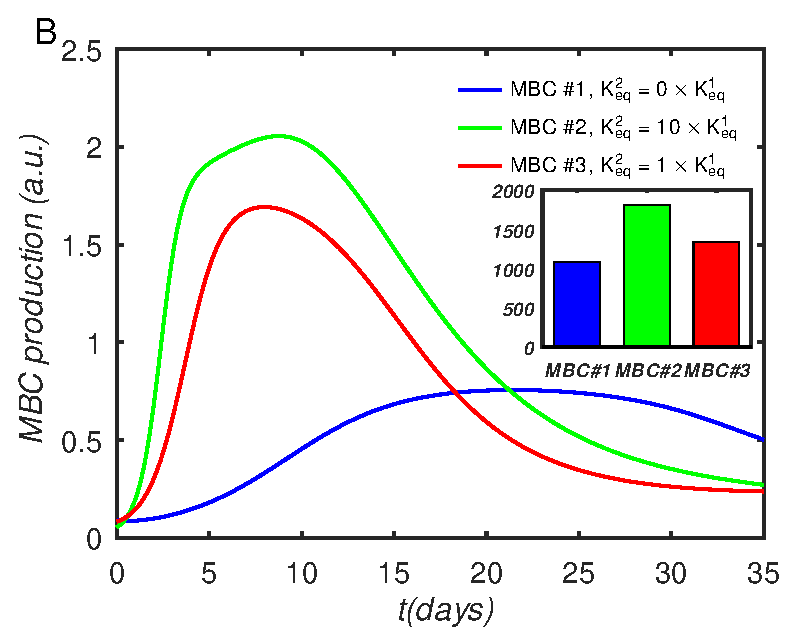
\includegraphics[width=0.49\textwidth]{../figS6/dmbc.eps}
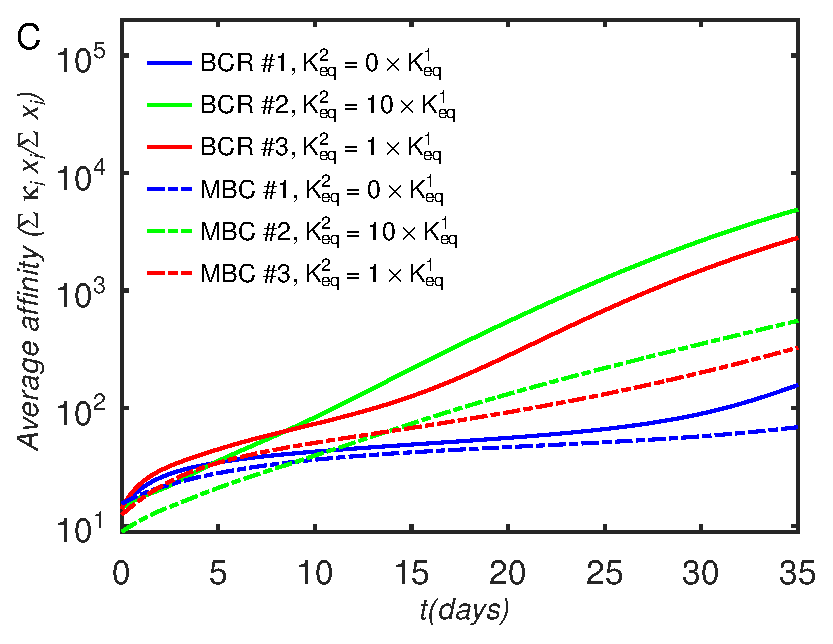
\includegraphics[width=0.49\textwidth]{../figS6/A.eps}
\caption{Effect of BCR valency and epitope concentration on GC evolution in the noninteracting regime ($o$=0);
$\alpha_1^T=2$, $\alpha_2^T=1$, $\alpha_3^T=1$; $\alpha^T$ is the nondimensional total Ag concentration.
Results for the fully interacting case are shown in Fig.~7 (main text).
}
\label{fig:agc0}
\end{figure*}

\vspace{1EM}
\subsection{
GC simulations of the effect of AG\#1 concentration with multiple competing BCRs}
\label{sec:fig7}

\begin{figure*}
\centering
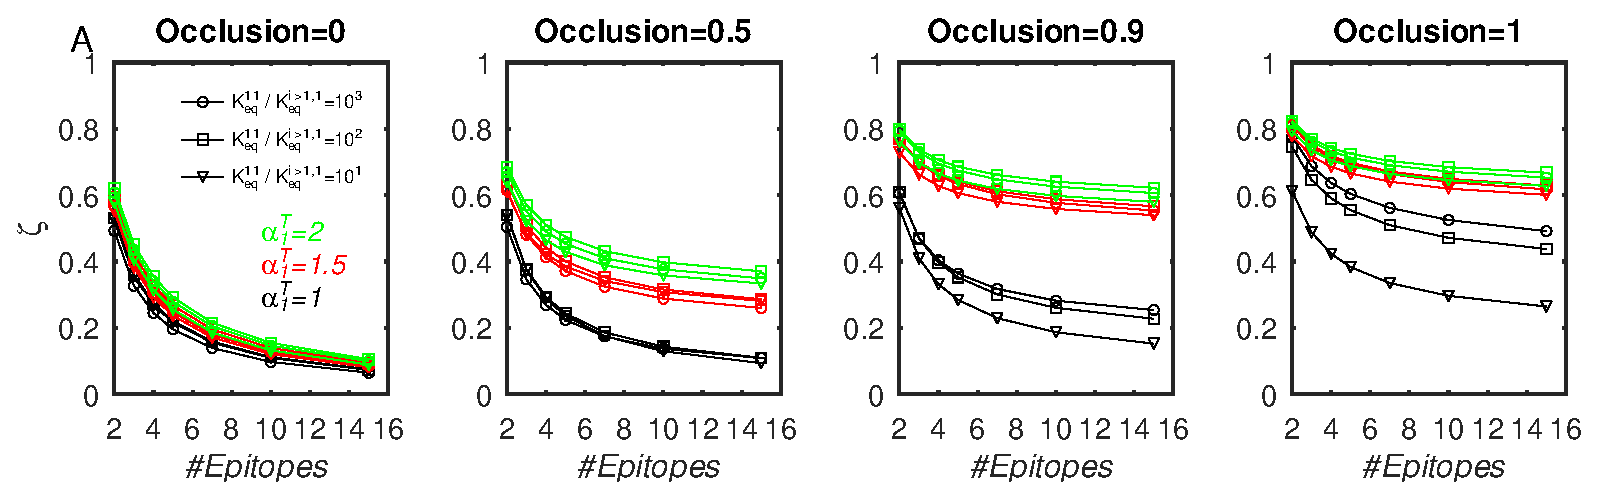
\includegraphics[width=0.99\textwidth]{../figS7/occl-k12=10.eps}
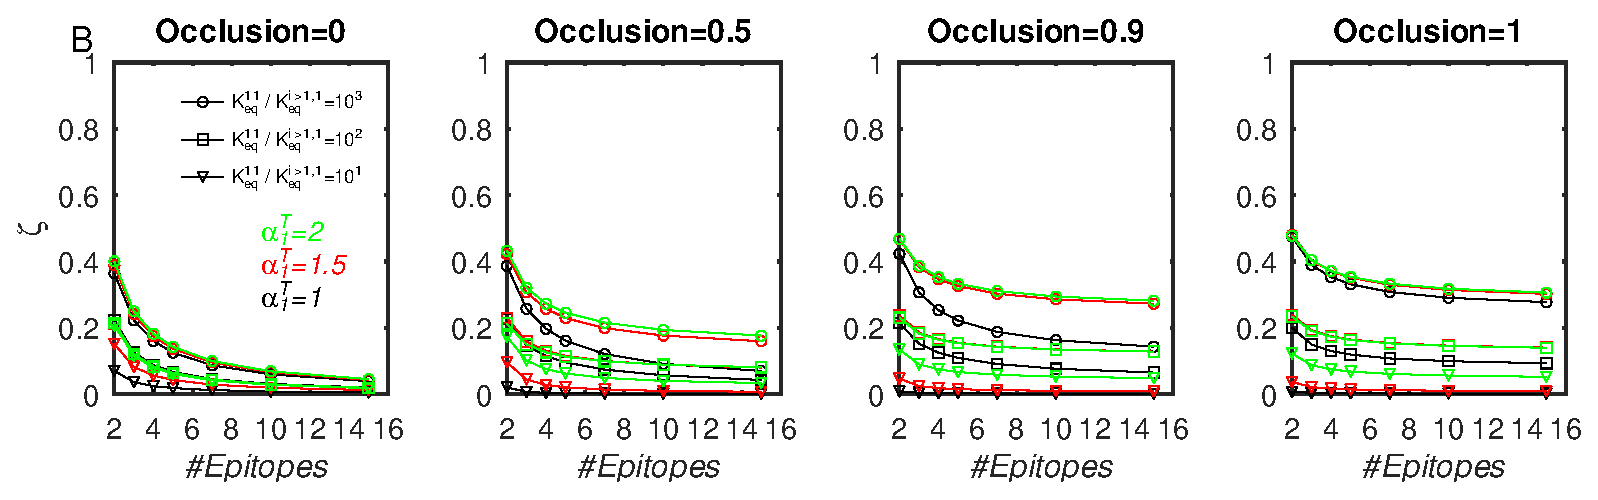
\includegraphics[width=0.99\textwidth]{../figS7/occl-k12=0.eps}
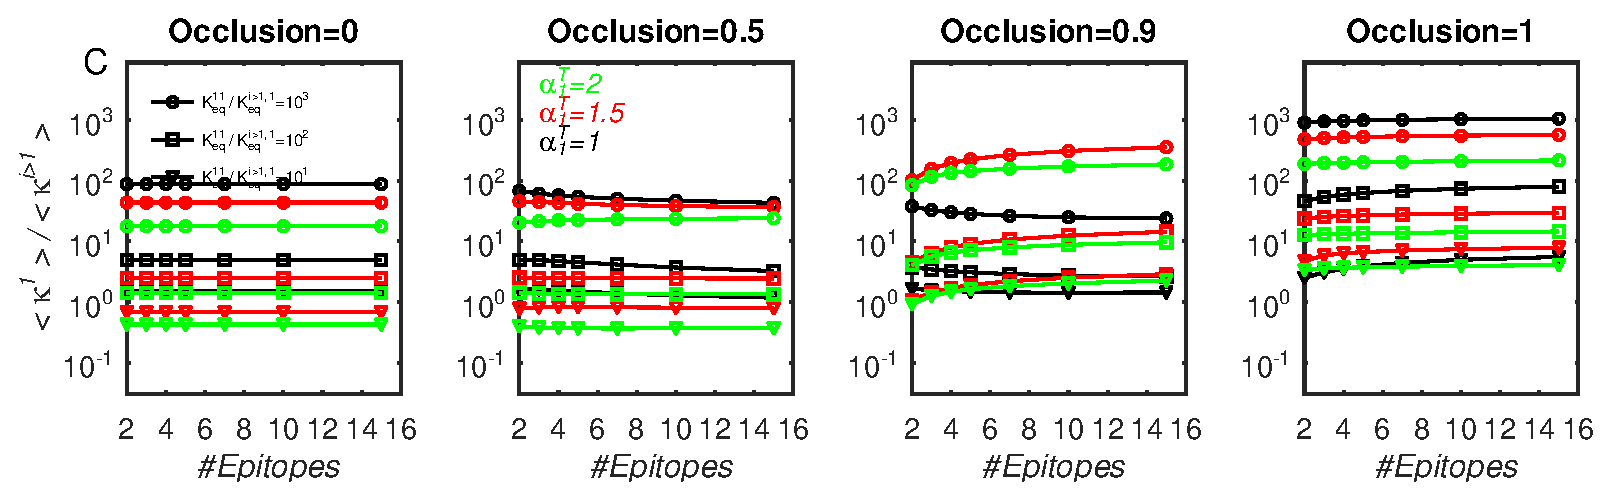
\includegraphics[width=0.99\textwidth]{../figS7/affr-k12=10.eps}
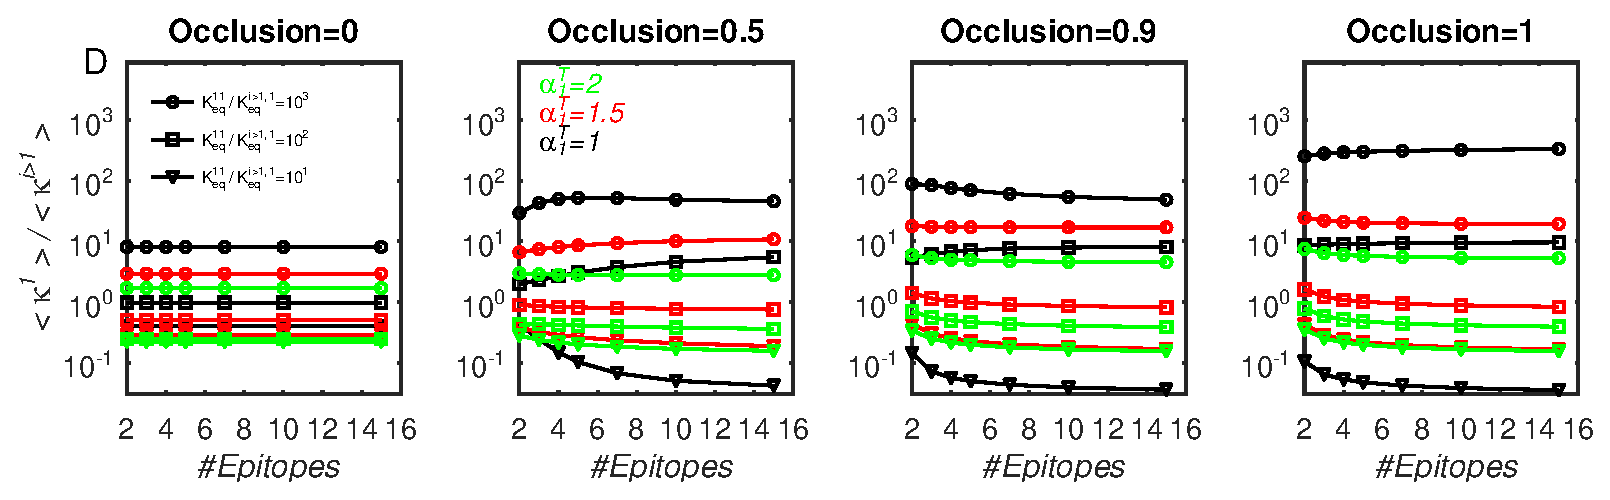
\includegraphics[width=0.99\textwidth]{../figS7/affr-k12=0.eps}
\caption{Results of six consecutive GC simulations with different initial affinity advantage values and epitope concentrations
 \vs~total number of BCR/Epitope pairs.
A \& B: MBC\#1 fraction ($\zeta$) at the end of simulations.
C \& D: Ratio of average MBC\#1 affinity to that of the other MBCs (see text);
in A \& C: BCR\#1 is cooperatively bivalent ($K^{12}_{eq}$=10$K^{11}_{eq}$);
in B \& D: BCR\#1 is monovalent ($K^{12}_{eq}$=0).
}
\label{fig:agc1s}
\end{figure*}

In Fig.~7 of the main text, it was shown that the antigen concentration has a large effect on B-cell and memory cell
growth, as well as on the affinity of the corresponding BCRs. For brevity, we
only showed the results of a single calculation with
3 BCR/epitope pairs with occlusion $o$=1. In this section, we repeat the calculations while systematically varying the
number of BCR/epitope pairs (2--15), occlusion parameter (0, 0.5, 0.9, 1), affinity advantage provided to the
BCR\#1s ($\times10$, $\times100$, and $\times1000$), and whether BCR\#1s bound monovalently
($K^{12}_{eq}$=0) or bivalently ($K^{12}_{eq}$=10$K^{11}_{eq}$). The
results are summarized in \fig{agc1s}, after six consecutive GC simulations, with the relative MBC\#1 output
shown in figures \fig{agc1s}A,B and average MBC\#1 affinity, relative to that of the other MBCs, in \fig{agc1s}C,D.
The average affinity of MBC lineage $i$ is computed as
$\langle\kappa^i\rangle= \sum_{j=1}^{N_\epsilon} \kappa^i_j w^i_j / \sum_{j=1}^{N_\epsilon} w^i_j$,
where $w^i_j$ and $\kappa_j^i$ are the nondimensional MBC concentrations and affinities, respectively
(see Methods).
For comparison, we also performed simulations with lower Ag\#1 amounts, \ie~$\alpha_1^T$=1 and $\alpha_1^T$=1.5 in
dimensionless units.

\Fig{agc1s} shows that increasing Ag concentration leads to a
greater MBC output in all cases, with the increase being larger if the
corresponding BCR also has a significant affinity advantage (shown for bivalent
and monovalent BCR\#1s in \Fig{agc1s}A and \Fig{agc1s}B, respectively).
The increased MBC output corresponds to decreased affinity, however, the affinity decrease
being larger for monovalent (\Fig{agc1s}D), rather than for bivalent
BCR\#1s (\Fig{agc1s}C). The simulation results therefore suggest that
epitope subdominance can be overcome by increasing epitope concentration
in vaccinations with cocktails of designed antigens, as proposed recently by
others,\cite{kanekiyo19,cohen21,glanville20} but at the expense of a
reduction in the affinity of the resulting MBCs.
For the practical purpose of vaccine design, the precise Ag concentrations
may need to be optimized to achieve a compromise between MBC population
size and affinity for antigen.\\

\begin{figure*}
\centering
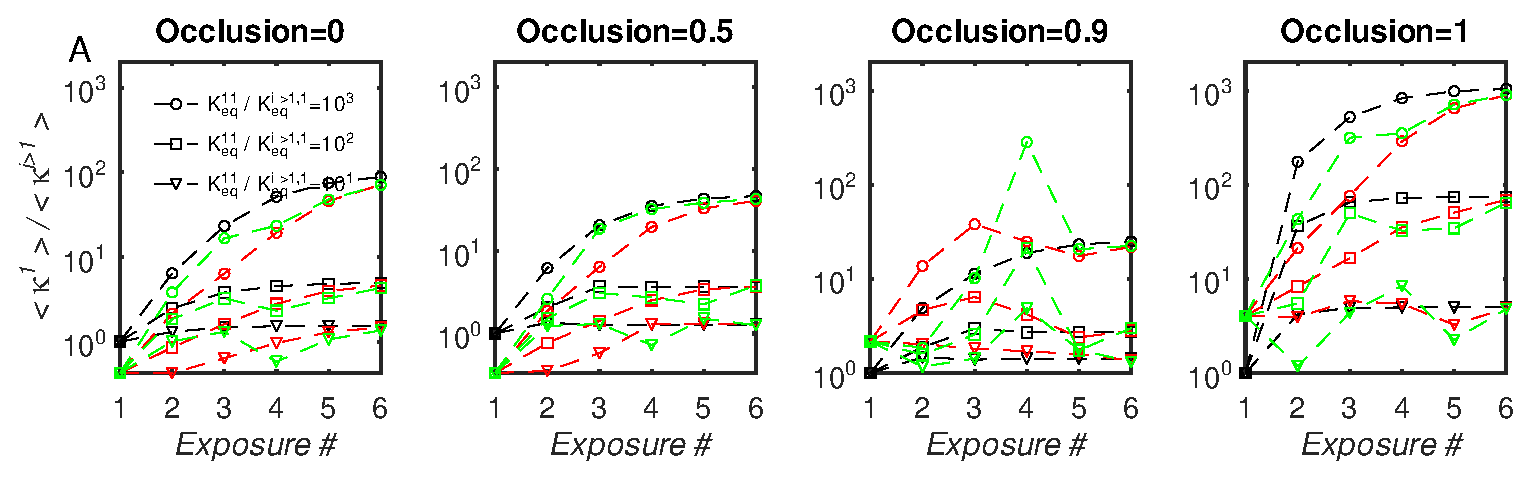
\includegraphics[width=0.99\textwidth]{../fig8-S3-S8/afftime-k12=10.eps}
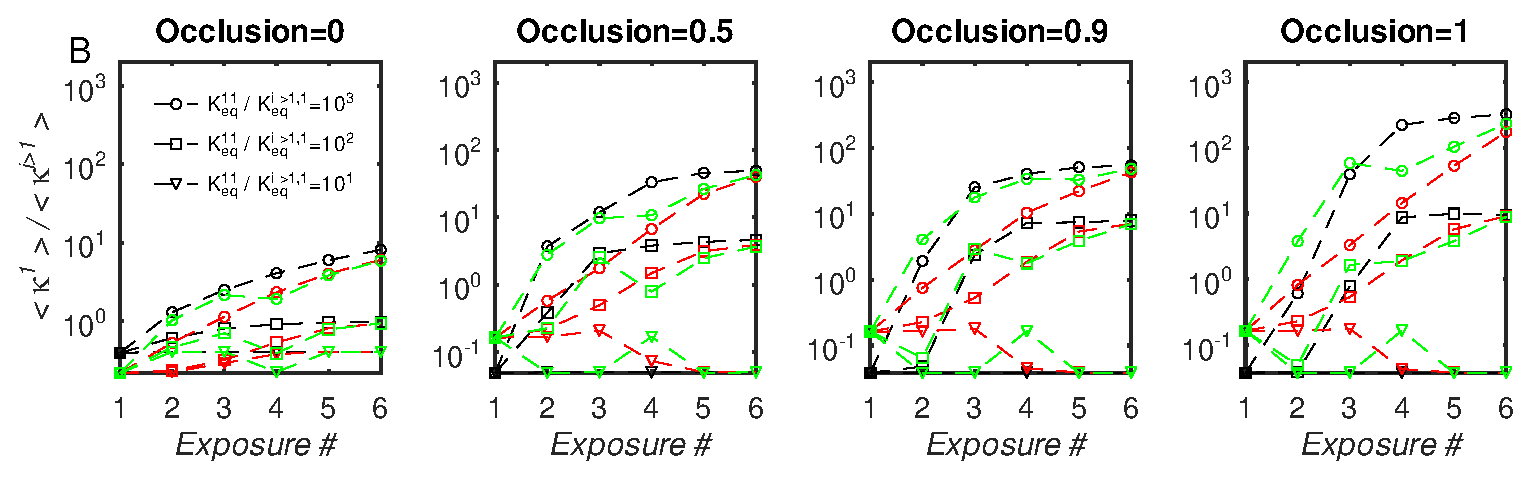
\includegraphics[width=0.99\textwidth]{../fig8-S3-S8/afftime-k12=0.eps}
\caption{Affinity of BCR\#1 \vs~number of sequential GC simulations for different initial affinity advantage values
and different AG\#1 concentrations, with 10 total BCR/Epitope pairs.
A \& B: Ratio of average MBC\#1 affinity to that of the other MBCs (see text);
A: BCR\#1 is cooperatively bivalent ($K^{12}_{eq}$=10$K^{11}_{eq}$);
B: BCR\#1 is monovalent ($K^{12}_{eq}$=0). The different colors correspond to different concentration profiles of Ag\#1, as given in the main text, and in 
Fig.~8A.
}
\label{fig:agtime2}
\end{figure*}

\vspace{2.5EM}
\subsection{Optimization of model parameters}
\label{sec:optim}
To optimize the fit of the model predictions to the experimental
data,\cite{wittenbrink11,weisel16} we used steepest (gradient) descent to
minimize the squared error (SE) between the simulated and
experimental GC size, MBC and PC production. To achieve similar weighting of the
errors from the GC, MBC and PC comparisons, each of the three SE components
was normalized by the corresponding mean-squared experimental value divided by the corresponding average experimental error bar.

The gradients of the SE with respect to a parameter, \eg~$\phi_i$, were obtained using the second-order finite difference formula,\ie
\begin{equation}
 \pd{SE}{\phi_i}^n \simeq \frac{SE(\phi^n_i+\delta\phi_i) - SE(\phi^n_i-\delta\phi_i)}{2\delta\phi_i},
 \label{eq:grad}
\end{equation}
where $\phi^n_i$ is the value of the parameter at optimization iteration $n$,
and $\delta\phi_i$ was the finite difference step set to 0.01.
Parameter values were updated using
\begin{equation}
 \phi^{n+1}_i = \phi^n_i - \Delta \times \pd{SE}{\phi_i}^n,
 \label{eq:update}
\end{equation}

where $\Delta\simeq 0.02$ was an empirically determined step size
chosen small enough to reduce instabilities, but large enough to achieve
relatively fast optimization, \eg~100 steps computed within $\sim$30 minutes of computer time.

The optimization described above is not very sophisticated, \eg,
conjugate gradient or Newton-Raphson minimization could be used to locate
optimal parameter values with greater accuracy and speed; however, the
simple steepest descent used here is sufficient for the present purposes,
because (1) the accuracy of the fit need only be within experimental
uncertainty, and (2) the optimization only needs to be performed once,
and therefore its speed of convergence is not very important.

\begin{figure*}[ht!]
\centering
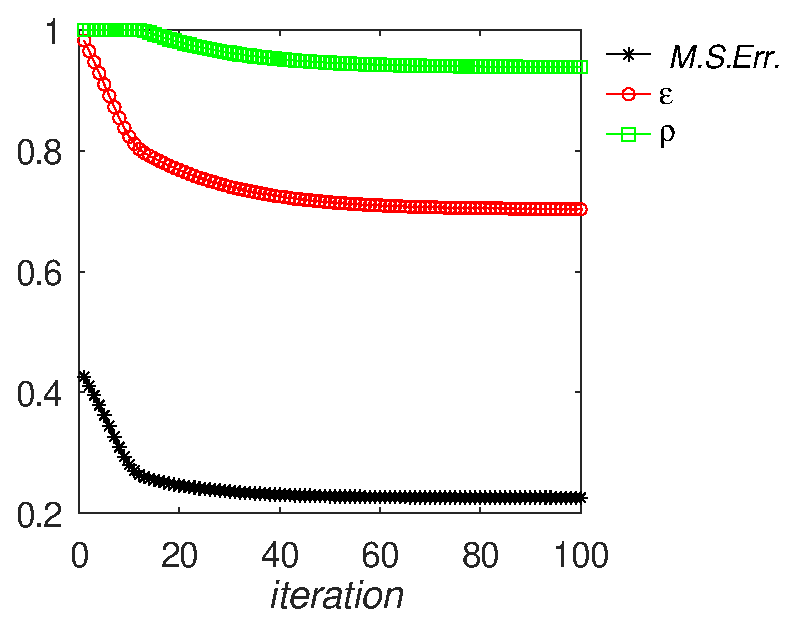
\includegraphics[width=0.45\textwidth]{../figS9/hfit.eps}
\caption{Illustration of parameter fitting using steepest descent minimization (see text).
}
\label{fig:optim}
\end{figure*}


In \fig{optim} we show the convergence of the parameters $\epsilon$ and $\rho$ in the activation function Eq.~10.
The values for both parameters were initially set to 1, and were constrained to the interval [0.5,1] by setting
any value that was outside the interval after an iteration, to the nearer boundary.
The optimization converges to $\epsilon\simeq 0.7$ and $\rho\simeq 0.94$ within about 100 iterations.
%; subsequent iterations
%result in oscillation, as is expected when the steepest descent minimizer is near a minimum; however, the parameters at iteration
%31 are already within the experimental uncertainty (see Fig.~3), indicating that further optimization is not needed.

\vspace{1EM}
\subsection{Activated proliferation model}
\label{sec:apm}
In Sec.~4 of the main text, we noted that the affinity maturation (AM) model used in this work implements
B-cell selection \via~rescue from apoptosis of B-cells with the highest affinity to their cognate epitope
(\aka~death-limited selection\cite{anderson09,zhang10,amitai17}). However, there is evidence that
B-cell activation actually increases the rate of proliferation of the corresponding B-cells in the
dark zone.\cite{gitlin15}

Mathematically, the activated model differs from the non-activated model (Eq.~2) in that the proliferation rate constant
is scaled by the activation function, \ie,
\begin{equation}
 \begin{aligned}
 \td{[B^i_j]}{t}=&\left\{-k_d(1-h^i_j) - k_p h^i_j\right\}[B^i_j] + 2k_p\sum^{N_\epsilon}_{k=1} m_{kj} [B^i_k]h^i_k,\\
  \textrm{for}\ 1\le& i\le N_B.
 \end{aligned}
 \label{eq:apam}
\end{equation}
\begin{figure*}
\centering
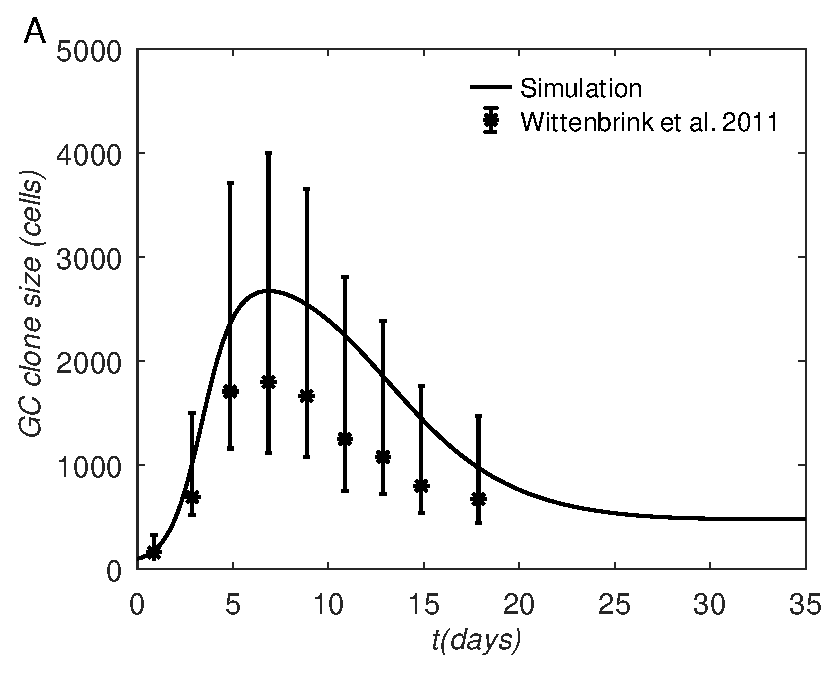
\includegraphics[width=0.32\textwidth]{../figS10/gcsize.eps}
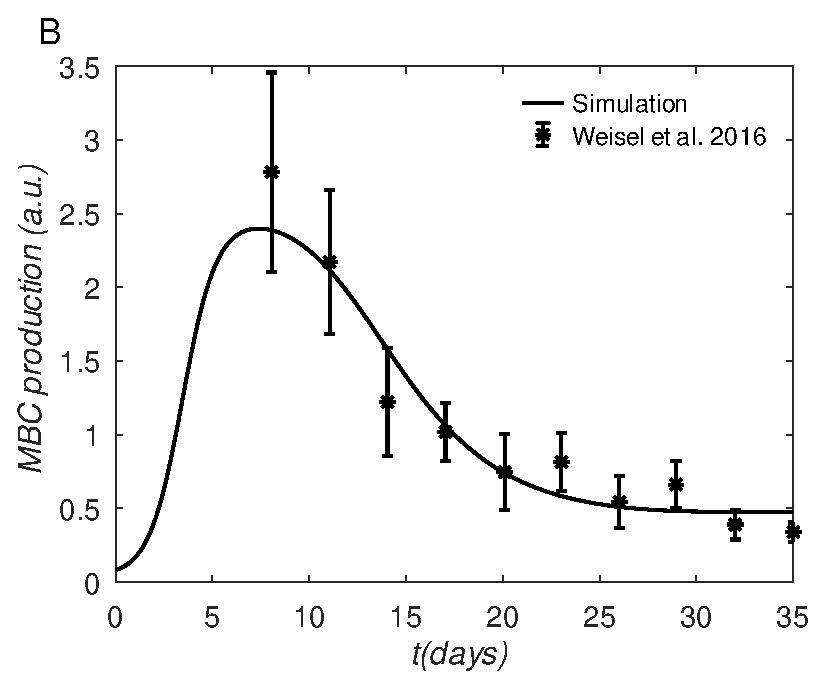
\includegraphics[width=0.32\textwidth]{../figS10/dmbc.eps}
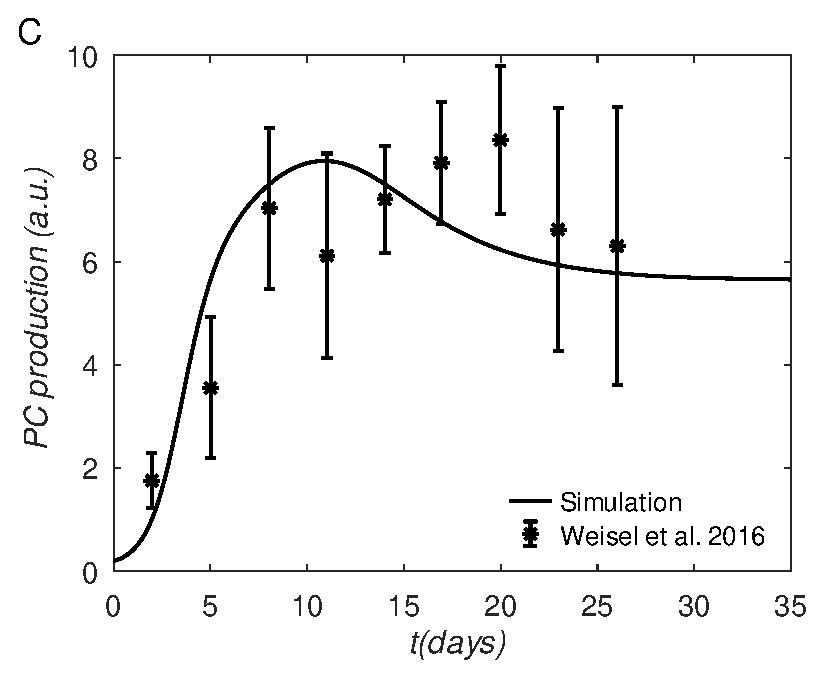
\includegraphics[width=0.32\textwidth]{../figS10/dplc.eps}
\caption{Comparison of experiments and simulations using the activated proliferation model (see text).
A: Total B cells, B: Memory cell production rate, C: Plasma cell
production rate. Experimental data for A was generated from the GC
cross-sectional areas plotted in Fig.~S1B of Ref.~\citenum{wittenbrink11}, and converted to B cell counts
as done in Ref.~\citenum{pelissier20};
experimental data for B \& C was taken from Fig.~4 of Ref.~\citenum{pelissier20}, who
used raw data from \citet{weisel16}.
}
\label{fig:apvalid}
\end{figure*}
\begin{figure*}
\centering
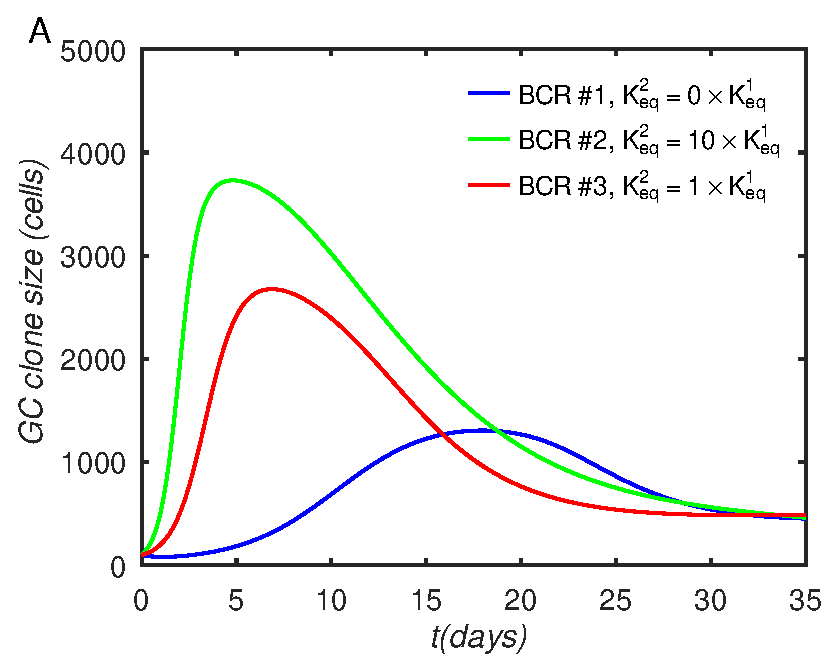
\includegraphics[width=0.45\textwidth]{../figS11abc/gcsize.eps}
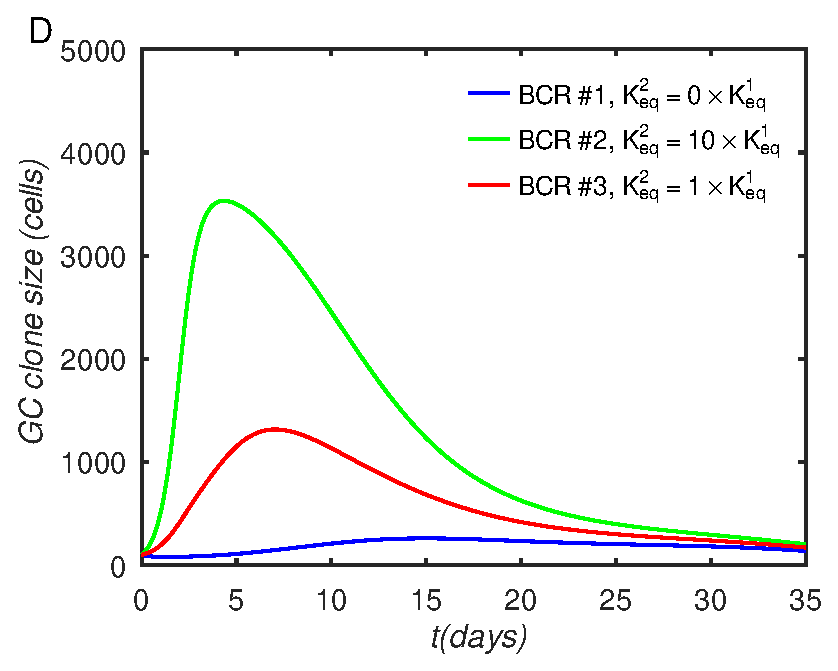
\includegraphics[width=0.45\textwidth]{../figS11def/gcsize.eps}
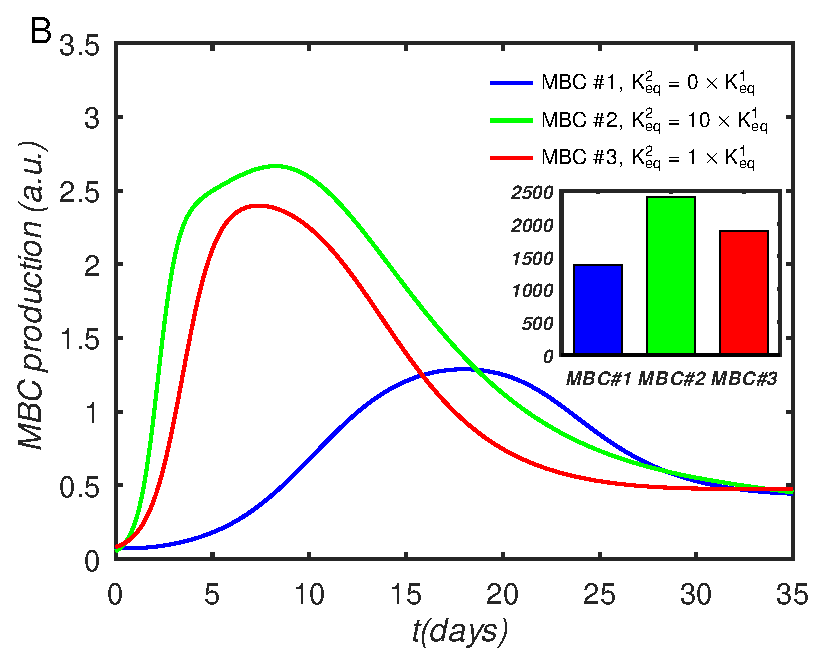
\includegraphics[width=0.45\textwidth]{../figS11abc/dmbc.eps}
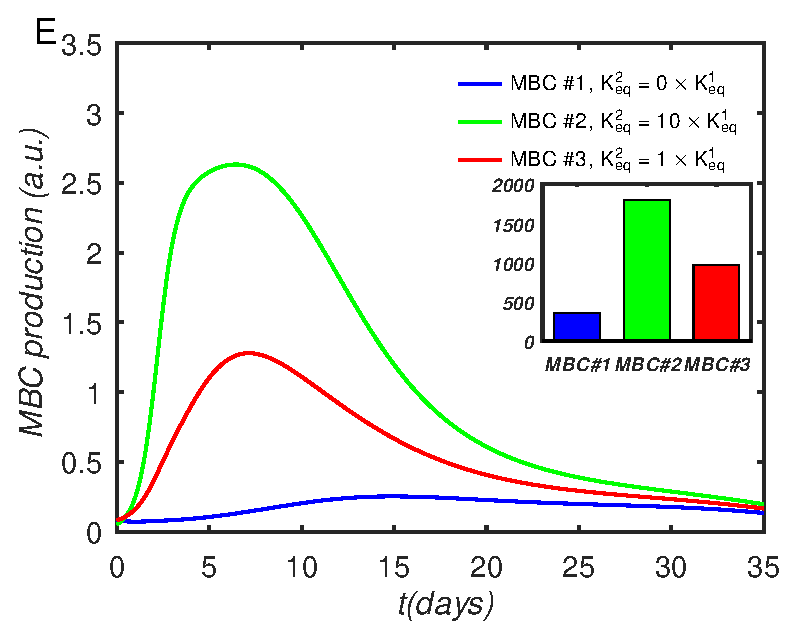
\includegraphics[width=0.45\textwidth]{../figS11def/dmbc.eps}
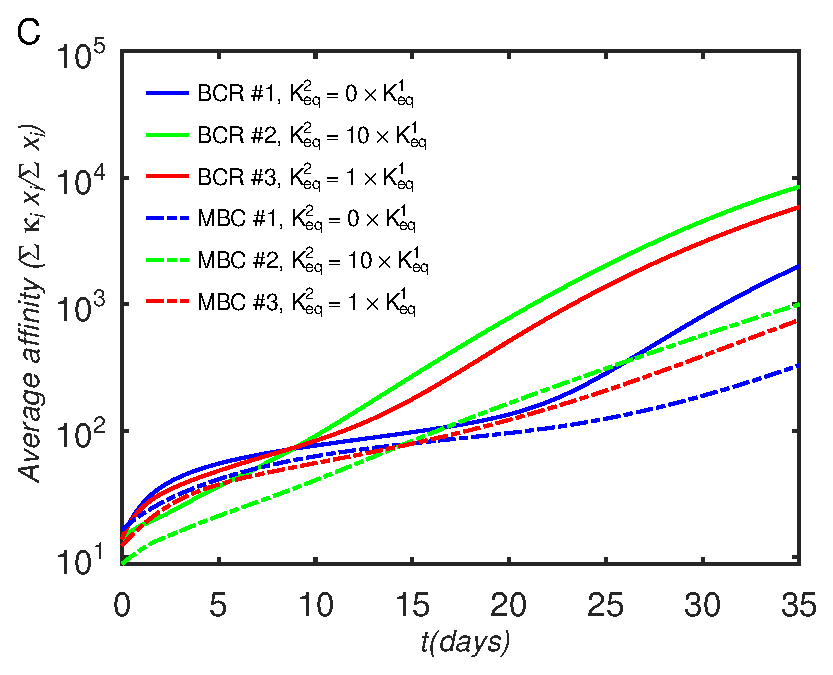
\includegraphics[width=0.45\textwidth]{../figS11abc/A.eps}
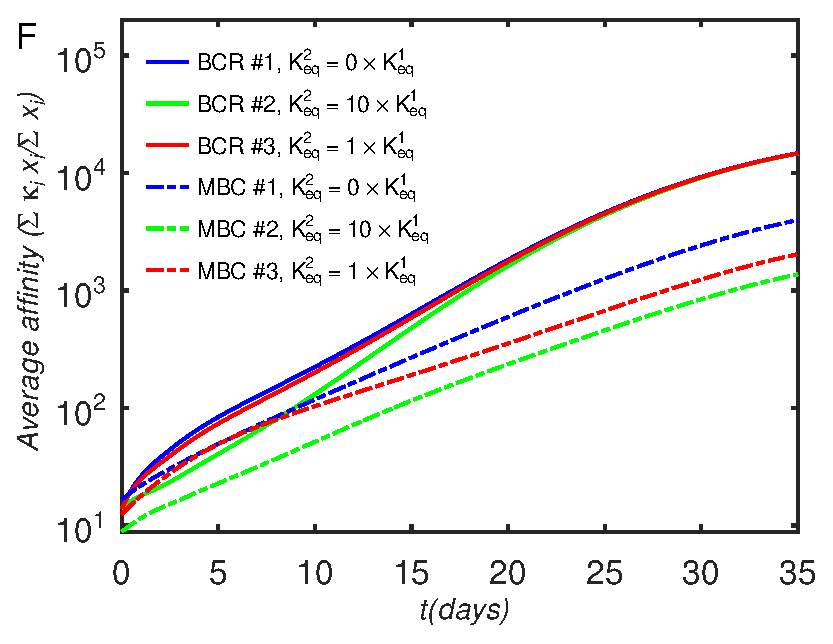
\includegraphics[width=0.45\textwidth]{../figS11def/A.eps}
\caption{Effect of antibody valency and epitope occlusion on GC properties. Simulated using the activated proliferation model.
Left column (A--C): noninteracting B-cell case ($o=0$);
Right column (D--F): fully interacting B-cell case ($o=1$);
A,D: Total B cells;
B,E: Memory cell production rate; insets: total MBC population at end of simulation;
C,F: Average affinity of B-cells and MBCs.
}
\label{fig:apavidity}
\end{figure*}
Because the modeling described here involves substantial fitting and
parametrization, and because the experimental data has high
uncertainties,\cite{wittenbrink11,weisel16} it was possible to fit the
data within the experimental uncertainties with either model. In \fig{apvalid}, we show the validation
calculations performed with one Ag using the activated proliferation
model. All of the simulation constants and parameters were kept as in
Table~1, except for modifications to the proliferation and death
rate constants that were needed to obtain a good fit to the experiment;
specifically~$k_p^{max}$=2.55/d, and $k_d$=2.25/d.
In partcular, the sizeable decrease in $k_d$ was needed to compensate for a
decrease in the proliferation rate caused by scaling the rate constant $k_p$ by 
the activation factor $h^i_j$, which is always below 1.

Compared with the results of the non-activated proliferation model in
Fig.~3 (main text), the maximum B-cell population is higher, but
remains well within the experimental dispersion.

Furthermore, we repeated several simulations with multiple BCR/Ag
pairs to check that our conclusions remained qualitatively the same.
For example, in \fig{apavidity} we show the results of simulating three
BCR/Ag pairs evolving independently ($o=0$, \fig{apavidity}A--C),
\vs~evolving while fully interacting with each other ($o=1$,
\fig{apavidity}D--F). Comparing the results with those derived from the
non-activated model (Fig.~4 in the main text), it is clear that the two models 
are in agreement in terms of the relative ranking of the cells according to population size or affinity. 

Thus the results suggest that the choice of activated \vs~nonactivated
proliferation is not likely to impact qualitatively the conclusions in this study.

\vspace{1EM}
\subsection{T-cell-dependent B-cell activation}
\label{sec:tcell}
A key component in the GC model presented here is the activation function
$h$, which determines which B-cells are rescued from apoptosis (Eq.~2)
or, in the case of activated proliferation, receive a proliferation advantage.
%
In the simulations described in the main text, we assumed that $h$ has a
simple dependence on the fraction of bound BCR Fabs (see
%\eqs{theta}{act}). However, the survival of B-cells also depends on
Eqs.~(8) and (10)). In reality, the survival of B-cells also depends on
the extent of their interactions with helper T-cells
(Tfh),\cite{liu89,allen07,crotty14} and thus it is desirable to have available a more realistic model of
activation that treats these interactions. In this
section, we describe a simple T-cell model related to that of \citet{mayer19}, and use it to compute a T-cell-based
function $h_T$, as a replacement for $h$ in Eq.~10. We
compare the outcomes of trial AM simulations performed with $h$
\vs~$h_T$, and conclude that the use of $h_T$ would not change
qualitatively the conclusions of this study. However, the model could be
used as a starting point for future studies, \eg, of the effects of changing T-cell
concentration, or other properties that could impact Tfh and B-cell
survival and proliferation.

We assume that each B-cell $B^i_j$ has a constant total number of major
histocompatibility complexes of type II ($MHC2^T$) which can be
unloaded ($MHC2^{i0}_j$) or loaded with an Ag-derived peptide ($MHC2^{iL}_j$).
The total concentration of MHC2's in the GC available for binding a T-cell receptor (TCR) is 
\begin{equation}
 [MHC2^T] =MHC2^T\times \sum_{j=1}^{N_\epsilon}\sum_{i=1}^{N_B}[B_j^i],
\end{equation}
and the corresponding total loaded and unloaded MHC2 concentrations are
\begin{equation}
 [MHC2^L]=\sum_{j=1}^{N_\epsilon}\sum_{i=1}^{N_B}[B_j^i] \times MHC2^{iL}_j,
\end{equation}
 and
\begin{equation}
 [MHC2^0]=[MHC2^T]-[MHC2^L],
\end{equation}
respectively.

We now postulate that unloaded and loaded MHC2's can bind to a TCR with equilibrium binding constants $K^T_0$ and $K^T_L$, respectively.
Given a total concentration of TCRs $[T^T]$, the unbound TCR concentration obeys a TCR conservation equation
analogous to Eq.~9\cite{kepler93}:
\begin{equation}
 [T] + [MHC2^L] \theta^T_L + [MHC2^0] \theta^T_0 = [T^T],
\label{eq:tcons}
\end{equation}
where
\begin{equation}
 \theta^T_L = \frac{ K^T_L [T] }{ 1 + K^T_L [T] },
\end{equation}
and
\begin{equation}
 \theta^T_0 = \frac{ K^T_0 [T] }{ 1 + K^T_0 [T] }
\end{equation}
are the fractions of loaded and unloaded MHC2 receptors, respectively, that are bound to a TCR.
Since we assume that there are only two types of MHC2 receptors (loaded and unloaded),
\Eq{tcons} is \vo{equivalent} to a quadratic polynomial in $[T]$, with the
solution\cite{mayer19}
given by the quadratic formula.

Solving \eq{tcons} requires the setting of
several parameters. First, we specify $MHC2^{iL}_j$ and $MHC2^{i0}_j$ using the following simplifying
assumptions: (1) the fraction of loaded MHC2's is equal to the the fraction of bound BCR arms, \ie,
\begin{equation}
 \frac{MHC2^{iL}_j}{MHC2^T}=\theta^i_j,
\end{equation}
and (2) we initially set the total number of MHC2 molecules displayed on
the B-cell surface to the number of BCRs (\ie~$\sigma$ in Table~1).
However, this number had to be empirically reduced to $10^4$ (10\% of the
number of BCRs) to match the experimental
observation that the GC T-cell population is below $\sim$20\% of the
total GC size\cite{allen07}. We note that there does not seem to be a biological justification for this reduction,
which may therefore indicate a deficiency in the model.

Second, we need to specify the MHC2/TCR binding constants $K^T$. To
set $K_L^T$ to a reasonable value, we assume that the maximum TCR-bound
fraction of MHC2 at saturating antigen and a physiological helper T-cell
concentration $[T^T]$ (to be specified below) is $\theta^T_{max}$=0.9.
In this regime, we approximate $[MHC2^0]\simeq 0$, and attribute the bound MHC2 fraction entirely
to peptide-loaded MHC2, which implies
\begin{equation}
 \theta^T_{max} = \theta^T_L.
 \label{eq:hmax}
\end{equation}
Solving \eq{hmax} for $K_L^T$ and eliminating $[T]$ using \eq{tcons} gives
\begin{equation}
 K_L^T=\frac{\theta^T_{max}}{([T^T]-\theta^T_{max} [MHC2^T])(1-\theta^T_{max})}.
 \label{eq:kt1}
\end{equation}
Similarly, we assume that when antigen is depleted, the TCR-bound fraction of MHC2, which in this case is
attributable to unloaded MHC2, is $\theta^T_{min}=0.01=\theta^T_0$. Solving for $K_0^T$ yields
\begin{equation}
 K_0^T=\frac{\theta^T_{min}}{([T^T]-\theta^T_{min} [MHC2^T])(1-\theta^T_{min})}.
 \label{eq:kt0}
\end{equation}

To compute the actual $K^T$ values, we assume the total T-cell concentration $[T^T]$ to be 200 cells, or $\sim$10\% of the average
GC peak of \citet{wittenbrink11}, which is roughly consistent with GC imaging.\cite{allen07} Further, we assume that maximal
binding cannot occur when $[MHC2^T]$ exceeds $[T^T]$, so we can set $[MHC2^T]=[T^T]$ in \eqs{kt1}{kt0}. With these assumptions,
\begin{equation}
 K_L^T=\frac{\theta^T_{max}}{[T^T] (1-\theta^T_{max})^2}=4.5\times 10^{-1}/cell
\end{equation}
and
\begin{equation}
 K_0^T=\frac{\theta^T_{min}}{[T^T] (1-\theta^T_{min})^2}=5.1\times 10^{-5}/cell.
\end{equation}

For each B-cell, the TCR-bound fraction is given by
\begin{equation}
 \theta^{iT}_j = \theta^T_L \theta^i_j + \theta^T_0 (1-\theta^i_j),
\end{equation}
where the first and second terms on the right-hand side represent contributions from loaded and unloaded MHC2's, respectively.
To use the T-cell-dependent B-cell activation model, we replace $\theta^i_j$ with $\theta^{iT}_j$ in Eq.~10.

We now consider the evolution of helper T-cells inside the GC. We assume that the T-cells whose receptors bind MHC2 complexes
on B-cells undergo increased proliferation. Specifically,
\begin{equation}
 \td{[T^T]}{t} = k^T_p \left([T^T]-[T]\right) - k^T_d [T^T],
 \label{eq:tdyn}
\end{equation}
where $k^T_p=1.25/d$ and $k^T_d=0.25/d$ are T-cell proliferation and death constants, respectively, which were manually adjusted 
from the T-cell model of \citet{mayer19}, who used $k^T_p=1.5/d$ and $k^T_d=0.2/d$, to improve agreement with experimental data.

We note that the above model of the effects of T-cells on GC dynamics is
heavily coarse grained, both spatially and temporally. For example,
B-cells and T-cells interact preferentially in the light zone, and
the duration, as well as the number of distinct encounters appear to be
important.\cite{allen07} These behaviors are captured to some extent in more complex
models,\cite{meyer-hermann12,pelissier20} but not in ours.  Further, only a single type of TCR is
included here, which does not discriminate between the different peptide
antigens that can be presented on MHC2s. However, increased model
complexity would require additional experimental data for parametrization and
validation.  Because they are not available, we restrict ourselves to 
qualitative-level predictions in this study.

\begin{figure*}
\centering
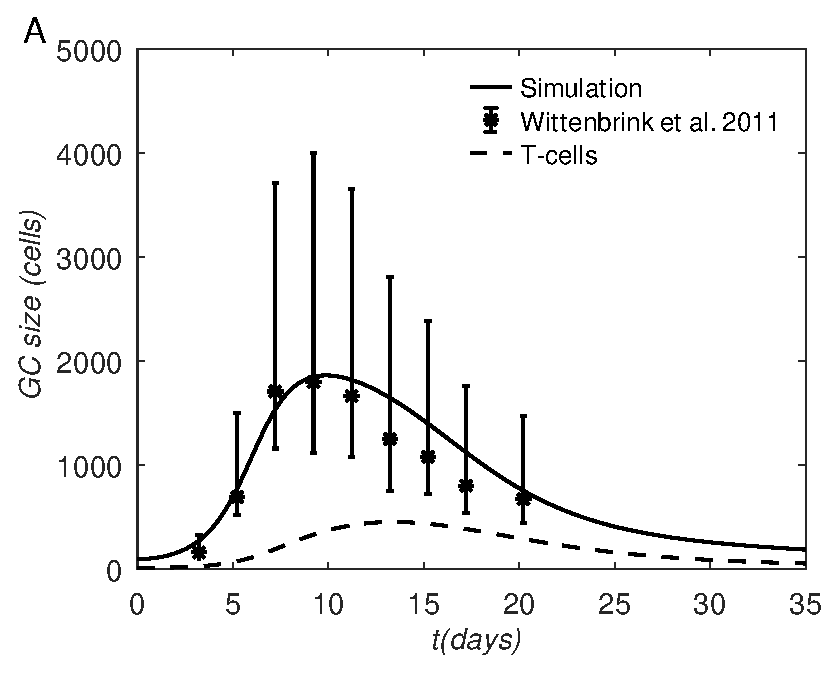
\includegraphics[width=0.325\textwidth]{../figS12/gcsize.eps}
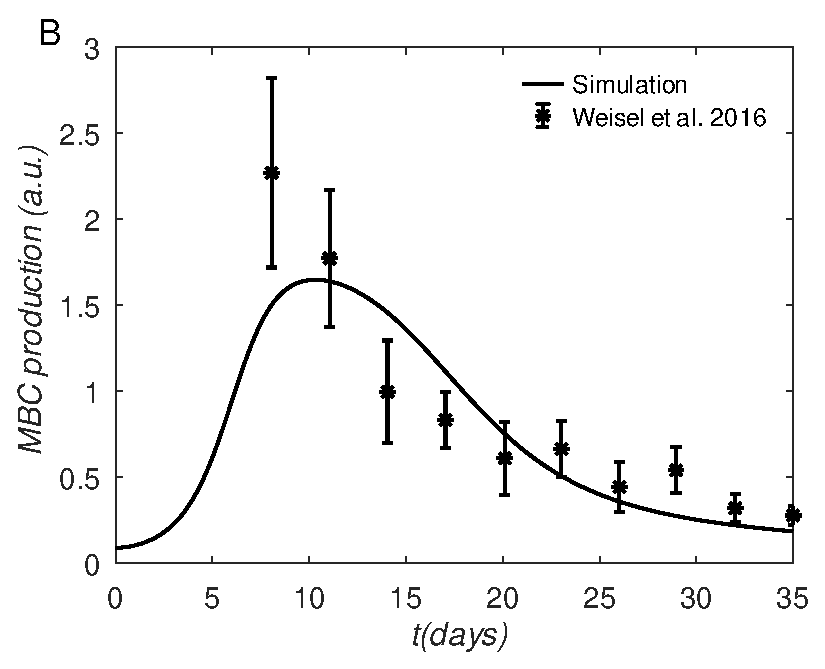
\includegraphics[width=0.325\textwidth]{../figS12/dmbc.eps}
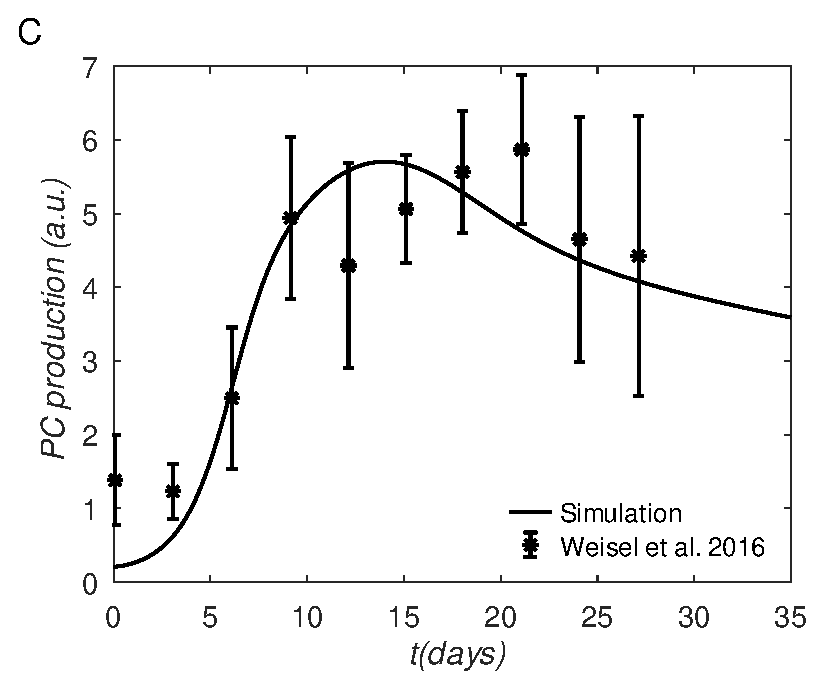
\includegraphics[width=0.325\textwidth]{../figS12/dplc.eps}
\caption{Comparison of experiments and simulations using the T-cell help model with non-activated proliferation (see text).
A: B-cells and T-cells, B: Memory cell production rate, C: Plasma cell
production rate.
}
\label{fig:tcvalid}
\end{figure*}

\begin{figure*}
\centering
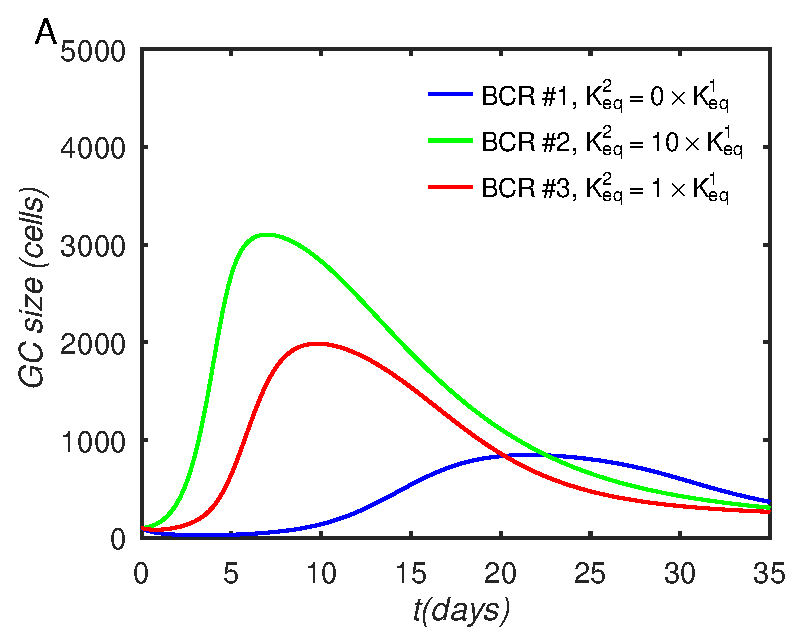
\includegraphics[width=0.45\textwidth]{../figS13abc/gcsize.eps}
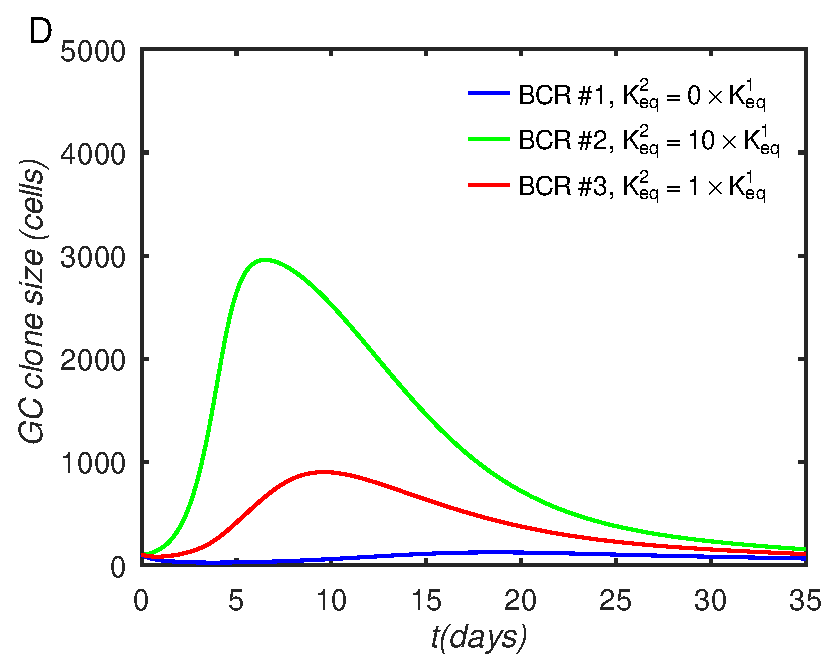
\includegraphics[width=0.45\textwidth]{../figS13def/gcsize.eps}
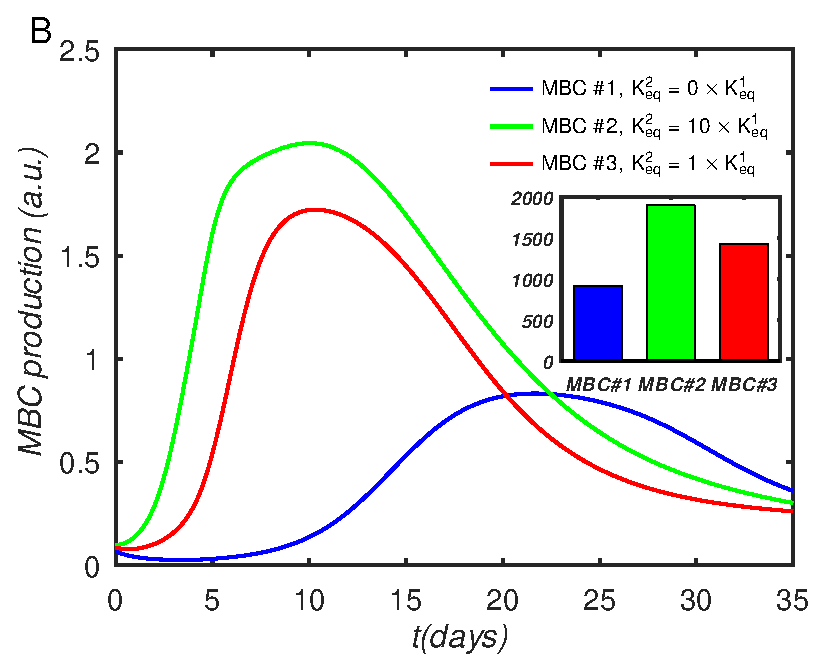
\includegraphics[width=0.45\textwidth]{../figS13abc/dmbc.eps}
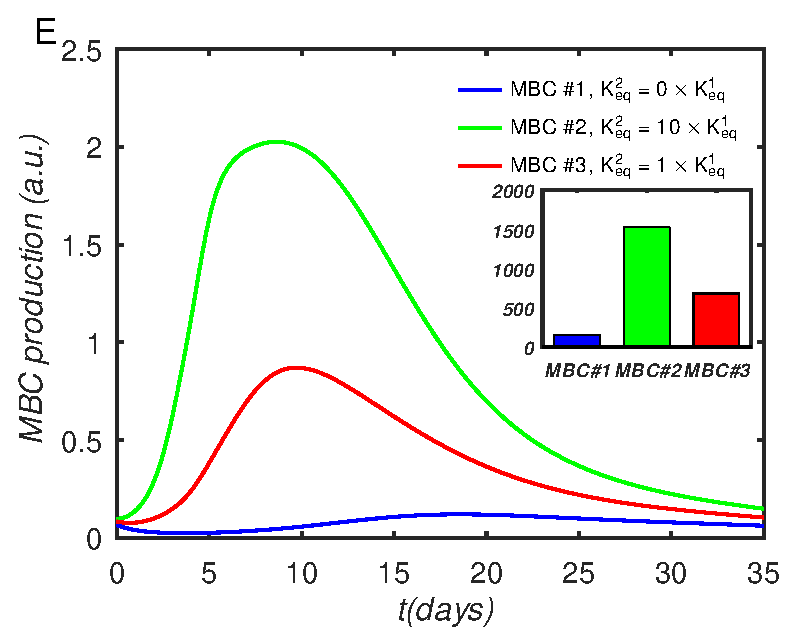
\includegraphics[width=0.45\textwidth]{../figS13def/dmbc.eps}
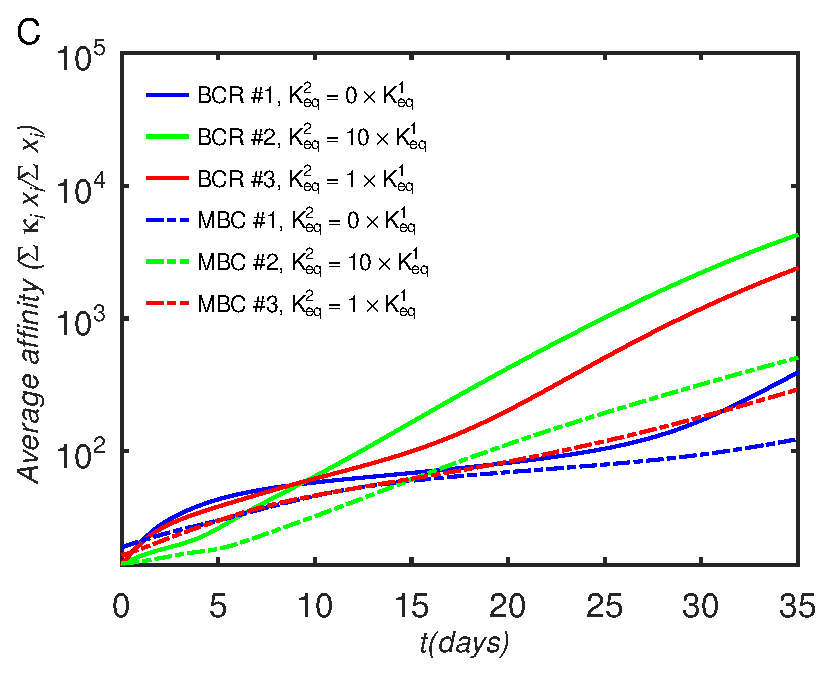
\includegraphics[width=0.45\textwidth]{../figS13abc/A.eps}
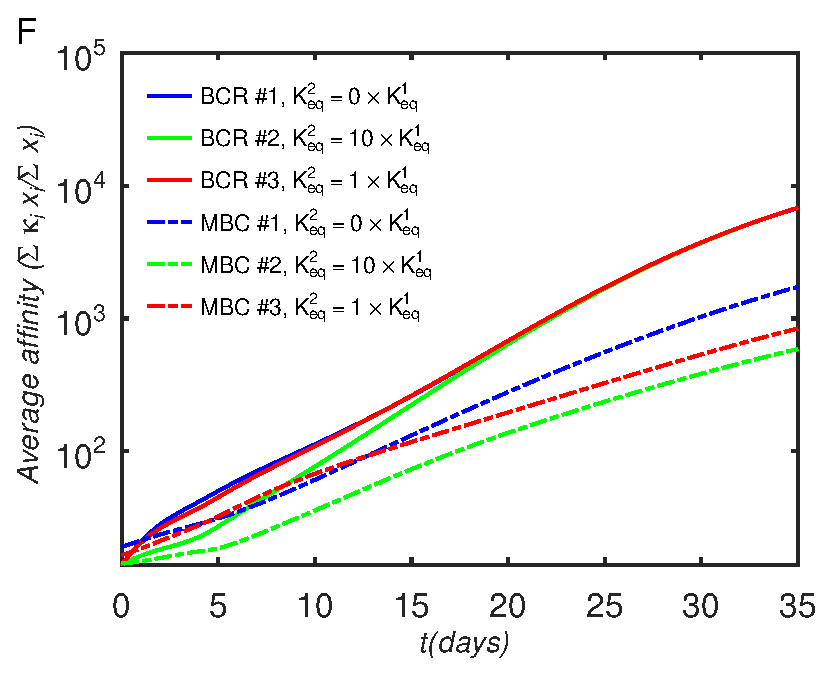
\includegraphics[width=0.45\textwidth]{../figS13def/A.eps}
\caption{Effect of antibody valency and epitope occlusion on GC properties.
Simulated using T-cell model with non-activated proliferation.
Left column (A--C): noninteracting B-cell case ($o=0$);
Right column (D--F): fully interacting B-cell case ($o=1$);
A,D: Total B cells;
B,E: Memory cell production rate; insets: total MBC population at end of simulation;
C,F: Average affinity of B-cells and MBCs.
}
\label{fig:tcavidity}
\end{figure*}

We first use the T-cell model to repeat the validation calculations of
the single-AG case. Aside from the use of the T cell model, all
simulation parameters were kept the same as in Table~1.
In \fig{tcvalid}, we show the total B and T cells (panel A), MBC production (panel B)
and PC production (panel C). Comparing with the results of the Ag-only activation model
(see Fig.~3 in the main text), the main difference is a $\sim$2 day delay in
the growth of all quantities. The reason for the delay is the extra time
required for T-cell expansion, before sufficient B-cell activation can take place.
The initial T-cell population was set to
10 cells, corresponding to 10\% of the initial B-cell population. The peak
T-cell population reached about 400 cells at 12 days, or 20\% of the maximum B-cell population of $\sim$2000 cells, which is
qualitatively consistent with known GC composition.\cite{allen07}

Next, in \fig{tcavidity} we show the results of GC simulations of three
BCR/Ag pairs, in the interacting and non-interacting cases, as was done
in Fig.~4 (main text) for the Ag-activated model. Comparison of
the two figures shows that the results are qualitatively the same.
Therefore, the use of the present T-cell model throughout would not be expected to
change the conclusions of this study. A possible explanation for the lack of
significant differences between the Ag-activated and T-cell activated
simulation results is that, in both cases, the models were first calibrated to
match the same experimental data. Furthermore, the activation provided by
the T-cell model ultimately comes from BCRs binding to Ags, \ie, it is
implicitly Ag-activated. While more complicated T-cell models would
likely cause larger differences in the GC population predictions, our
objective in this study was to only investigate the robustness of our
predictions of the effects of BCR/Ag valency on B-cell competition with respect to
changes to the GC model.
